\documentclass[conference]{IEEEtran}
\IEEEoverridecommandlockouts
% The preceding line is only needed to identify funding in the first footnote. If that is unneeded, please comment it out.
% \usepackage{cite}
\usepackage{amsmath,amssymb,amsfonts}
\usepackage{algorithmic}
\usepackage{graphicx}
\usepackage{subcaption}
\usepackage{textcomp}
\usepackage{xcolor}

% alternative citation package
\usepackage[
  backend=biber,
  sorting=none,
  style=ieee,
  % doi=false,
  % isbn=false,
  url=false,
  eprint=false
]{biblatex}
\addbibresource{refs.bib}

% additional packages
\usepackage[colorlinks]{hyperref}
\hypersetup{
    colorlinks,
    citecolor=black,
    filecolor=black,
    linkcolor=black,
    urlcolor=black
}
% mathematical fonts and graphics
\usepackage{bm} % bold fonts in math mode
\usepackage{mathtools}
\usepackage{xfrac} % sfrac for diagonal slashes in fractions
\usepackage{amsfonts} % math fonts
\usepackage{amssymb} % more math symbols (supsetneq etc.)
\usepackage{dbnsymb}
\usepackage{dsfont} % math fonts
\usepackage{bbm} % mathbb fonts
\usepackage{mathrsfs} % fancy swirly font
\usepackage{gensymb} % degree sign
\usepackage{cancel} % cancel terms
% plots
\usepackage{pgfplots}
\usepackage{pgfplotstable}
\usepgfplotslibrary{external}
\usepgfplotslibrary{patchplots}
\usepgfplotslibrary{groupplots}
\pgfplotsset{compat=1.18} 
\tikzexternalize[prefix=tikz,optimize=false]

% ~~~~~~~~~ MATH MACROS ~~~~~~~~~~~~~~~~~~~~~~~~~~~~~~~~~~~~~~
\newcommand\abs[1]{\left|#1\right|}
\newcommand\abss[1]{\left|\left|#1\right|\right|}
\newcommand\norm[1]{\left\lVert#1\right\rVert}
\newcommand\angled[1]{\left\langle#1\right\rangle}
\newcommand\round[1]{\left\lfloor#1\right\rceil}
\newcommand\dist[1]{\left|\left|#1\right|\right|}
\newcommand\arr[1]{\left\langle#1\right\rangle}
\newcommand\pdpi[0]{\frac{\partial}{\partial p_i}}
\newcommand*\Laplace{\mathop{}\!\mathbin\nabla^2}
\newcommand\vek[1]{\vec{\bm{#1}}}
\newcommand\nvek[1]{\hat{\vec{\bm{#1}}}}
\newcommand\mat[1]{{\mathds{#1}}}
\newcommand\br[1]{\left(#1\right)}
\newcommand\abr[1]{\left\langle#1\right\rangle}
\DeclareMathOperator{\sgn}{sgn}
\DeclareMathOperator{\erf}{erf}
\DeclareMathOperator*{\argmax}{\arg\!\max}
\DeclareMathOperator*{\argmin}{\arg\!\min}
\newcommand\divergence{{\nabla\cdot}}

% fancy boxes
\usepackage{fancybox}
\newcommand{\equationnamed}[2]{%
  \setlength{\fboxsep}{2pt} % padding inside box
  \setlength{\fboxrule}{0.01pt}
  \begin{center}
    \begin{minipage}{\linewidth}
      \begin{center}\textsc{#1}\end{center}
      #2
    \end{minipage}
  \end{center}
}
\newcommand{\equationnamedbox}[2]{%
  \setlength{\fboxsep}{5pt} % padding inside box
  \setlength{\fboxrule}{0.01pt}
  \begin{center}
    \fbox{
      \begin{minipage}{0.92\linewidth}
        \begin{center}\textsc{#1}\end{center}
        #2
      \end{minipage}
    }
  \end{center}
}

% % Glossary
% \usepackage[acronym]{glossaries}
% \makenoidxglossaries
% % technical
% \newacronym{ppe}{PPE}{Pressure Poisson Equation}
% \newacronym{sph}{SPH}{Smoothed Particle Hydrodynamcs}
% \newacronym{cfl}{CFL}{Courant-Friedrichs-Lewy}
% % methods
% \newacronym{iisph}{IISPH}{Implicit Incompressible SPH}
% \newacronym{pcisph}{PCISPH}{Predictive-Corrective SPH}
% \newacronym{pbf}{PBF}{Position Based Fluids}
% \newacronym{dfsph}{DFSPH}{Divergence-free SPH}

\usepackage{acronym}



\def\BibTeX{{\rm B\kern-.05em{\sc i\kern-.025em b}\kern-.08em
    T\kern-.1667em\lower.7ex\hbox{E}\kern-.125emX}}
% replacement for the above for bibtex:
\renewcommand*{\bibfont}{\normalfont\fontsize{8}{10}\selectfont}
% \renewcommand*{\bibfont}{\normalfont\footnotesize}


\begin{document}


\title{Optimal SPH Pressure Fields using Quadratic Programs\\
% {\footnotesize \textsuperscript{*}Note: Sub-titles are not captured in Xplore and
% should not be used}
% \thanks{Identify applicable funding agency here. If none, delete this.}
}

\author{\IEEEauthorblockN{Julian Karrer}
\IEEEauthorblockA{\textit{Department of Computer Science} \\
\textit{University Freiburg}\\
Freiburg, Germany \\
julian.karrer@students.uni-freiburg.de}
}

\maketitle

\begin{abstract}
The problem of finding the least pressure field that satisfies the continuity equation for incompressible fluids in accordance with Gau\ss's principle of least constraint is modelled as an optimization problem for fields that are discretized using Smoothed Particle Hydrodynamics. This yields a series of one convex Quadratic Programs per time step that robustly computes optimal pressure values for SPH-based simulation of incompressible, low-viscosity fluids.\textsl{}
\end{abstract}

\begin{IEEEkeywords}
Optimization, QP, SPH, fluid dynamics, PMPG
\end{IEEEkeywords}

\section{Introduction}
\ac{sph} is a popular Lagrangian discretization scheme for problems in continuum mechanics that is used extensively for the simulation of fluids in Computer Graphics. In animation in particular, Newtonian, nearly incompressible fluids with low viscosity such as water are of interest, and a core challenge in their simulation is strongly enforcing the incompressibility of the fluid without incurring visual artefacts such as volume loss and oscillations. One scalar pressure value per fluid particle must be computed such that the fluid remains in an uncompressed or divergence-free state, leading to the formulation and solution of the pressure Poisson equation. Conventional pressure solvers attempt to minimize compression with respect to some inequality constraints imposed by the discretization scheme, but they are typically designed to find any feasible solution, not an optimal or least solution in any sense. This in turn can lead to sensitivity of the solution to implementation details and initialization, where aggressive warm-starting for example can lead to instabilities and excessive pressure forces might result. The aim of this report is to instead formulate the problem of pressure computation as an optimization problem, where the least pressure field in the sense of physical action is computed, yielding a physically plausible and robust result independent of initialization and solver implementation as a series of convex \ac{qps}. While the efficient solution of the resulting \ac{qps} for large systems is not the focus of this report, the resulting pressure solver can already serve as a baseline for the verification of correctness of the implementation of other pressure solvers, as demonstrated in \autoref{sec:results}.\\

This report will outline the governing equations of the dynamics to be simulated in continuous form before introducing the discretization schemes applied to the resulting problem, all the while exploring the deliberate choices of source terms, integration scheme, kernel functions, approximations of differential operators, time step sizes, linearizations, simplifying assumptions etc. made along the way. Each choice is justified with reference to the literature and preferably kept uncontroversial such that the report may serve as a proof of concept of maximum applicability to existing \ac{sph} simulations. This should also give the context required to appreciate not just the stated final optimization formulation but understand the choices that have led to it. Finally, the resulting optimization problem is analysed and solved using an interior point method, as well as compared to existing incompressible \ac{sph} pressure solvers for fluid simulation.





\section{Governing Equations}
\subsection{Navier Stokes Equations in Continuous Form}
The problem of simulating the flow of a Newtonian fluid on macroscopic scales can be formulated in terms of continuum mechanics, where the time evolution of field quantities, or functions of time and space, and their deformation is described. In this setting, flow is governed by the Navier-Stokes equations, a set of partial differential equations that will be outlined here in their Lagrangian or non-conservation form, which means that quantities are described with respect to the moving frame of reference of infinitesimal fluid elements that are advected along with the velocity field $\vek{v}\br{\vek{x}, t}$, as opposed to an Eulerian view of the problem which describes the flux of quantities as they move through a reference frame that is fixed in space, which would lead to the so-called conservation form of the equations \cite{anderson}. 
The Lagrangian Navier-Stokes equations consist of the \emph{momentum equation} \cite{tutorial2019}:
\equationnamed{Momentum Equation}{
    \begin{equation}\label{eq:momentum}
        \vek{a} = \frac{D\vek{v}}{Dt} = -\frac{1}{\rho}\nabla p + \nu \Laplace \vek{v} + \vek{b}^\text{ext}
    \end{equation}
}
which describes how the velocity field $\vek{v}$ evolves in time due to accelerations $\vek{a}$ comprised of internal viscous and pressure accelerations as well as accelerations caused by external body forces $\vek{b}^\text{ext}$ acting on the fluid while preserving linear and angular momentum, as well as the \emph{continuity equation} that expresses conservation of mass \cite{anderson}:
\equationnamed{Continuity Equation}{
  \begin{equation}\label{eq:continuity}
    \frac{D\rho}{Dt} = -\rho\br{\divergence \vek{v}}
  \end{equation}
}
where $\rho$ is density, $p$ is pressure and $\nu=\frac{\mu}{\rho}$ is the kinematic viscosity that is closely related to the dynamic viscosity $\mu$. In this setting, the only external acceleration acting on each volume $\vek{b}^\text{ext}=\vek{g}$ is gravity.

Note that the dependence of fields on time and space as well as each other is customarily omitted in the notation unless relevant to the discussion (e.g. when quantities at a time $t+\Delta t$ different from the current time $t$ are predicted), more precise definitions will follow in the discretized context. The operator $\frac{D}{Dt}$ is referred to as the material derivative or substantial derivative, which quantifies the instantaneous time rate of change of quantities measured in the reference frame of an advected fluid element: in a Lagrangian setting, this conveniently simplifies to the local derivative $\frac{\partial}{\partial t}$, while in an Eulerian setting an additional convective derivative $\vek{v} \cdot \nabla$ must be accounted for since the movement of the fluid element past a fixed point in space might induce a rate of change of an advected quantity at a fixed position \cite{anderson}. 

The continuity equation plays a particularly central role for incompressible fluids, where $\frac{D \rho}{D t} = -\rho\br{\divergence \vek{v}}\overset{!}{=} 0$ holds, the product in which allows a decomposition into equivalent incompressibility constraints, any one of which must be enforced \cite{survey2022}:
\begin{align}
    \divergence \vek{v} = 0 & \quad\textit{divergence-free velocity field}\label{eq:source-div-free}\\
    \frac{D \rho}{D t} = 0  & \quad\textit{no change in density (differential)}\label{eq:source-rho-diff}\\
    \rho = \rho_0           &\quad \textit{no change in density (absolute)}\label{eq:source-rho-abs}
\end{align}

While these constraints are equivalent in a continuous setting, they differ in a time-discretized implementation since any numerical errors incurred will accumulate and manifest in different ways. While the former two constraints are based on differential or flux quantities with respect to time and space and errors will therefore accumulate as drift, or in this case irrecoverable volume loss, \autoref{eq:source-rho-abs} is an absolute reformulation of \autoref{eq:source-rho-diff} where density can be computed from the primary quantity of mass that can be perfectly conserved in a Lagrangian setting, so errors will instead manifest as oscillations of the density field about the field with constant rest density $\rho_0$. Since such a Lagrangian, particle-based framework will be used, the implementation of the third constraint is straightforward, whereas in an Eulerian setting where flux quantities are tracked with respect to a computational grid that is fixed in space, the first constraint is a more natural choice. 
% Direct enforcement of \autoref{eq:source-rho-diff} appears to be rarely attempted in \ac{sph}-based settings \cite{survey2022}.

% In a discrete time setting with time steps of size $\Delta t$, \autoref{eq:source-rho-diff} and \autoref{eq:source-rho-abs} are often combined in some form equivalent to:
% \begin{equation}
%     \rho(t) + \Delta t \frac{D\rho}{Dt}(t) = \rho_0\label{eq:source-den-invariant}
% \end{equation}
% where numerical integration yields a predicted density at $t+\Delta t$ on the left-hand side, reconstructed from both the absolute density at $t$ and the local instananeous rate of change of density at $t$ due to velocity divergence.

Depending on the constraint or constraints implemented, the resulting source term for pressure computation is called density-invariant (\autoref{eq:source-rho-abs}) or divergence-free (\autoref{eq:source-div-free}). SPH-based pressure solvers ubiquitously use the density-invariant formulation \autocites{iisph}{pcisph}{dfsph}{optimized-source-term}{pbf}: the manifestation of numerical errors as oscillations is generally seen as much less problematic than drift, even more so in settings with non-negligible viscosity, which can help damp such oscillations. 
In this report, the density-invariant source term will therefore be the focus.
However, some methods such as \ac{dfsph} \cite{dfsph} and variations of the \ac{iisph} method \cite{optimized-source-term} combine iterations with divergence-free and density-invariant forms of the continuity equation as source terms for pressure computation in order to exploit both the superior quality of the resulting velocity field from \autoref{eq:source-div-free} as well as prevent degrading of the sampling quality by using \autoref{eq:source-rho-abs} \cite{optimized-source-term}.

Finally, the kinematics of the system follow Newton's equations of motion, where positions $\vek{x}$ and velocities $\vek{v}$ are described by a set of ordinary differential equations:
\begin{equation}\label{eq:eqs-of-motions}
  \begin{split}
    \ddot{\vek{x}} &= \dot{\vek{v}} = \vek{a}\\
    \dot{\vek{x}} &= \vek{v}
  \end{split}
\end{equation}

\subsection{Temporal Discretization and Numerical Integration}\label{sec:time-discretization}
To make simulation of the system tractable, continuous time must be discretized into finite time steps of some size $\Delta t$. This time step size need not be fixed over the course of a simulation but can be set dynamically to a value that balances accuracy and computational performance, however it is upwards bound by the \ac{cfl} necessary condition for convergence of the simulation to the solution of the \acs{pdes} \cite{survey2022}:
\begin{equation}\label{eq:cfl}
    \Delta t \leq \lambda \frac{h}{\abss{\vek{v}^\text{max}}}
\end{equation}
for the parameter $\lambda \in (0,1)$, commonly set to $\lambda=0.4$ \cite{survey2022}\cite{sph-monaghan-92}, the maximum velocity $\vek{v}^\text{max}$ and a particle diameter $h$. This means that a particle shall not move further than the spatial unit of the \ac{sph}-discretization per time step, which makes intuitive sense. In the implementation underlying this report, a conservatively small, constant time step size was chosen to rule out any source of error in implementation and ensure the CFL condition is always upheld, however this choice is not particularly relevant to the following discussions.

Given a time step size $\Delta t$, the equations of motion from \autoref{eq:eqs-of-motions} can be numerically integrated. The integration method will become an inherent part of the problem formulation and many derived terms, so it is of some importance. Semi-implicit Euler integration (also known as symplectic Euler or Euler-Cromer) is a simple and computationally inexpensive first-order method that has favourable energy conservation properties over explicit Euler integration, so it is extremely popular \cite{tutorial2019} in \ac{sph} fluid solvers. It can be argued that since the critical time step size imposed by the \ac{cfl} condition on high-Reynolds incompressible flow is much lower than in weakly compressible or strongly viscous settings \cite{optimal-isph-timestep}, more computationally expensive higher order time integration schemes justified by larger time step sizes are not ideal. For this reason, symplectic Euler will be chosen in this report and reads \cite{survey2022}:
\begin{equation}\label{eq:semi-implicit-euelr}
  \begin{aligned}
    \vek{v}\br{t + \Delta t} &= \vek{v}(t) + \Delta t \vek{a}(t) & \textit{explicit update}\\
    \vek{x}\br{t + \Delta t} &= \vek{x}(t) + \Delta t \vek{v}\br{t + \Delta t} & \textit{implicit update}
  \end{aligned}
\end{equation}

Generally, explicit time integration relies only on known quantities at some current time $t$ and is computationally inexpensive, while a more costly implicit integration can massively improve stability for stiff systems in particular. A defining technique for most iterative \ac{sph} fluid solvers is the so-called \textit{operator splitting} of the momentum equation \cite{survey2022}. For incompressible fluids of low viscosity, the much stiffer pressure accelerations dominate viscous accelerations while gravity is constant and known, so \autoref{eq:momentum} is split into two summands to be solved separately and sequentially, yielding a predictor-corrector scheme \cite{survey2022}:

\begin{equation}\label{eq:operator-split-vel}
  \begin{aligned}
    \vek{v}^*(t) &= \vek{v}(t) +\underbrace{ \Delta t \br{\nu \Laplace \vek{v} + \vek{g}}}_{ \Delta t \vek{a}^{\nu,g}}\\
    \vek{v}\br{t + \Delta t} &= \vek{v}^*(t) \underbrace{- \Delta t \frac{1}{\rho}\nabla p}_{\Delta t \vek{a}^p}
  \end{aligned}
\end{equation}

When intermediate, predicted velocities $\vek{v}^*$ are known, pressure computation becomes the task of finding pressure gradients $\nabla p$ that cause pressure accelerations $\vek{a}^p$ which induce changes in velocity according to the numerical time integration scheme that was chosen, such that $\vek{v}^*$ is projected onto a divergence-free state \cite{survey2022}. In other words, pressures are computed such that incompressibility is upheld at the next time step, i.e. $\frac{D\rho}{Dt}\br{t+\Delta t}=0$. This is the core task of a \ac{sph} pressure solver and the point at which an optimization problem will arise upon closer inspection. 

% Note that while all fields are functions of time and space, $\frac{D\rho}{Dt}$ as defined in \autoref{eq:continuity} has a dependence on the velocity field, in this case on $\vek{v}^*$. 



% IDEA: compare neighbourhood deficiency to lack of partition of unity compared to Galerkin methods!


% \begin{enumerate}
%   \item Compute predicted velocities $\vek{v}^*$ due to explicitly integrated accelerations $\vek{v}^*(t) = \vek{v}(t) + \Delta t \br{\nu \Laplace \vek{v} + \vek{g}}$
%   \item Assuming $\vek{v}^*$, find $\nabla p$ such that incompressibility $\frac{D\rho}{Dt}=0$ is upheld at $t+\Delta t$
%   \item Compute final velocities $\vek{v}\br{t + \Delta t} = \vek{v}^*(t) - \Delta t \frac{1}{\rho}\nabla p$ to use in \autoref{eq:semi-implicit-euelr}
% \end{enumerate}



% Finally, a very popular trick that is applicable in a discrete time setting is the combination of incompressibility constraints derived from the continuity in \autoref{eq:source-rho-diff} and \autoref{eq:source-rho-abs} by integration of $\frac{D\rho}{Dt}$ over time to obtain a predicted density $\rho + \Delta t \frac{D\rho}{Dt}$, which yields:
% \begin{equation}\label{eq:predicted-rho}
%   \begin{aligned}
%     \rho_0  &= \rho + \Delta t \frac{D\rho}{Dt} &\text{\autoref{eq:source-rho-diff}, \autoref{eq:source-rho-abs}} \\
%             &= \rho - \Delta t \rho(\divergence \vek{v})&\text{\autoref{eq:continuity}}
%   \end{aligned}
% \end{equation}



\subsection{The Pressure Poisson Equation}

Pressure is a constraint force that is defined in this case by the incompressibility constraint $\frac{D\rho}{Dt}= -\rho(\divergence \vek{v})= 0$ where velocity at $t+\Delta t$ depends on the pressure field. Depending on which variation of the incompressibility constraint (\autoref{eq:source-div-free}, \autoref{eq:source-rho-diff}, \autoref{eq:source-rho-abs}) is chosen, a different source term for a resulting system of equations can be derived after operator splitting. In agreement with much of the literature, this report will focus on a density-invariant source term formulation based on \autoref{eq:source-rho-abs}. 

Ideally, one would demand that:
\begin{equation}
  \rho(t+\Delta t) = \rho_0
\end{equation}
however, it turns out that when space is discretized in \autoref{sec:sph}, density is computed as a non-linear function of particle positions, which themselves are an affine function in the unknown pressures but enter density through a smoothing kernel function. A solution of the \acs{nlp} that would result from this choice of constraint was attempted but did not yield promising results, as discussed in \autoref{sec:nlp-attempt}. To avoid the nonlinearity, one may instead linearize the constraint by Taylor-expansion of $\rho$ in time about $t$ and obtain an incompressibility constraint on a first-order approximated \textit{predicted density} $\rho^*(t+\Delta t)$ due to non-pressure accelerations, as is commonly done in practice \cite{survey2022}:
\begin{equation}\label{eq:rho-change-non-pr}
  \begin{aligned}
    \rho(t+\Delta t) &= \rho(t) + \Delta t\frac{D\rho}{Dt}(t)+ \mathcal{O}\br{\Delta t^2}&\textit{Taylor expansion}\\
    \rho^*(t+\Delta t) &:=  \rho(t) \underbrace{- \Delta t \rho(t)\br{\divergence \vek{v}^*(t)}}_{\Delta t\frac{D\rho}{Dt}(t)}&\textit{\autoref{eq:continuity} on $\vek{v}^*$}
  \end{aligned}
\end{equation}

From this, the difference between the predicted density and rest density $\Delta \rho_{\nu,g} = \rho^*(t+\Delta t) - \rho_0$ follows, which is precisely what must be corrected for by an equal and opposite change in density due to pressure accelerations ($\Delta \rho_p = -\Delta \rho_{\nu,g}$).

The change in density due to pressure accelerations $\Delta \rho_p$ can be derived as follows:
\begin{equation}\label{eq:rho-change-pr}
  \begin{aligned}
    \Delta t \vek{a}^p &= - \Delta t \frac{1}{\rho}\nabla p & \textit{from \autoref{eq:operator-split-vel}}\\
    \br{\frac{D\rho}{Dt}}^p &= -\rho\br{\divergence \br{- \Delta t \frac{1}{\rho}\nabla p}} & \textit{insert into \autoref{eq:continuity}}\\
    \Delta \rho^p &= -\Delta t\rho\br{\divergence \br{- \Delta t \frac{1}{\rho}\nabla p}} & \textit{integrate w.r.t time}\\
    &= \divergence \br{\nabla p} \Delta t^2 & \textit{simplify}\\
    &= \Delta t^2 \Laplace p&
  \end{aligned}
\end{equation}

Combining prediction and correction, one obtains the so-called \ac{ppe} with a density invariant source term:
\equationnamed{Pressure Poisson Equation}{
  \begin{equation}\label{eq:ppe-rho-invariant}
    \begin{aligned}
      \Delta t^2 \Laplace p &= \rho_0 - \rho^*(t+\Delta t)\\
      &= \rho_0 - \rho + \Delta t \rho\br{\divergence \vek{v}^*}
    \end{aligned}
    \end{equation}
}

If the divergence-free constraint from \autoref{eq:source-div-free} had been used, a similar derivation would yield \cite{survey2022}:
\begin{equation}
  \Delta t^2 \Laplace p = \rho\br{\divergence\vek{v}^*}
\end{equation}

So far, spatial discretization would yield a linear system of equations per time step in unknown pressure values, which could at most be considered an optimization problem if its solution is interpreted as the unconstrained minimization of a corresponding quadratic form, justifying the use of solvers such as \ac{cg}. However, more constraints and complications will follow from unfavourable properties of the \ac{sph} method, which is outlined in the following \autoref{sec:sph}.  

\section{Smoothed Particle Hydrodynamics}\label{sec:sph}
\subsection{Fundamentals}\label{sec:sph-fundamentals}
So far, the discussion has been limited to fields that are continuous in space, which is intractable for numerical simulation. As a discretization scheme, the \acl{sph} method, independently discovered by \autocite[Gingold and Monaghan]{sph-monaghan-92} and \autocite[Lucy]{sph-monaghan-92} in 1977 and originally used in Astrophysics will be applied. It is an interpolation scheme and a meshless colocation method that allows the reconstruction of continuous fields throughout space from their values at discrete points \cite{duarte-meshless}.

A brief and instructive derivation of the method can be given from the point of view of sampling theory. Consider the Dirac-$\delta$ distribution on $\mathds{R}^d$, defined to satisfy both $\forall x\in\mathds{R}^d: x\neq \vek{0} \Longrightarrow \delta\br{\vek{x}} = 0$ and $\int_{\mathds{R}^d} \delta\br{\vek{x}} \, d\vek{x} = 1$ as the limiting distribution of the Gaussian $\mathcal{N}\br{\vek{0}, \sigma^2}$ as $\sigma^2\to 0$ \cite{tutorial2019}. By the convolution theorem, since $\delta$ is the constant unit function in the frequency domain, for sufficiently smooth functions $f: \mathds{R}^d\to\mathds{R}$ the following identity holds \cite{tutorial2019}:
\begin{equation}\label{eq:dirac-ident}
  f\br{\vek{x}} = (f \ast \delta)(\vek{x}) = \int_{\mathds{R}^d} f(\vek{x}') \delta(\vek{x}- \vek{x}')\,d\vek{x}'
\end{equation}

This exact identity needs to be approximated in two key positions \cite{tutorial2019}:
\begin{enumerate}
  \item The continuous integral is approximated by a sum over finitely many discrete samples, in a \textit{particle approximation} \cite{liu2010}. Considering the sifting property of the Dirac-$\delta$, this leaves the convolved field only pointwise non-zero at $N$ particle locations $\vek{x}_i$ for $i\in\mathds{N}_1^N$. The integral approximation becomes more accurate as the sample resolution increases.
  \item An only pointwise non-zero field does not admit meaningful spatial derivates, let alone notions such as the computation of a density field from the mass field. Quantities sampled at, and associated with, particle location $\vek{x}_i$ are therefore interpolated or smoothed out across space, which is done by relaxing the Dirac-$\delta$ as a convolution kernel from $\lim_{\sigma^2 \to 0} \mathcal{N}\br{\vek{0}, \sigma^2}$ to any normalized kernel function $W$ with some smoothing length $\hbar$ that approaches the $\delta$-distribution as $\hbar\to 0$. This approximation gets more accurate as $\hbar$ decreases.
\end{enumerate}

The smoothing kernel function is typically denoted $W\br{\vek{x}, \hbar}: \mathds{R}^d\times\mathds{R}^+\to\mathds{R}$, which when applied to differences in particle positions $\vek{x}_{ij} := \vek{x}_i - \vek{x}_j$ is typically shortened to $W_{ij}:=W\br{\vek{x}_{ij}, \hbar}$ for constant $\hbar$. In this report, the widespread definition $\hbar:=2h$ in the particle diameter $h$ (which is taken to correspond to the initial particle spacing on a regular grid) is chosen. Field quantities of some field $f$ at position $\vek{x}_i$ are denoted $f_i := f(\vek{x}_i)$ \cite{tutorial2019}. The basic SPH approximation of some field $f$ at $\vek{x}_i$, denoted $\abr{f_i}$, follows from approximation of \autoref{eq:dirac-ident} and reads \cite{tutorial2019}:
\equationnamed{Classic \ac{sph} Sum}{
  \begin{equation}\label{eq:sph-sum-basic}
    \abr{f_i} = \sum_{j\in\mathcal{N}_i} V_j f_j W_{ij} = \sum_{j\in\mathcal{N}_i} \frac{m_j}{\rho_j} f_j W_{ij}
  \end{equation}
}
where use of $\sfrac{m_j}{\rho_j} = V_j$ is a matter of convention and $\mathcal{N}_i = \mathds{N}_1^N$ for non-compactly supported kernels $W$ (otherwise, see \autoref{eq:neighbour-set-def}).

Note that in particular, density can be computed from the perfectly conserved masses per particle and their positions directly as \cite{tutorial2019}:
\begin{equation}\label{eq:density-estimate}
\begin{aligned}
  \rho_i &= \sum_{j\in\mathcal{N}_i} \frac{m_j}{\rho_j} \rho_j W_{ij}\\
  &= \sum_{j\in\mathcal{N}_i} m_j  W_{ij}
\end{aligned}
\end{equation}

\subsection{Kernel Functions}
Two necessary properties of a smoothing Kernel $W$ for the validity of the approximation in \autoref{sec:sph-fundamentals} were already alluded to, namely the normalization- and Dirac-conditions \cite{tutorial2019}:
\begin{equation}
  \begin{aligned}
    \int_{\mathds{R}^d} W\br{\vek{x}, \hbar} \,d\vek{x} &= 1 & \textit{normalization}\\
    \lim_{\hbar\to 0} W\br{\vek{x}, \hbar} &= \delta\br{\vek{x}} & \textit{Dirac-condition}\\
  \end{aligned}
\end{equation}

Other properties that are commonly enforced include \cites{tutorial2019}{liu2010}:
\begin{equation}\label{eq:kernel-criteria}
  \begin{aligned}
    W\br{\vek{x}, \hbar} &\geq 0 & \textit{positivity}\\
    W\br{\vek{x}, \hbar} &= W\br{-\vek{x}, \hbar} & \textit{symmetry}\\
    W\br{\vek{x}, \hbar} &\in C^2 &\textit{smoothness\cite{liu2010}}\\
    \forall \vek{x}\in\mathds{R}^d: \abss{\vek{x}} > \hbar &\Longrightarrow W\br{\vek{x}, \hbar} = 0 & \textit{compact support}\\
  \end{aligned}
\end{equation}
In fact, spherical symmetry $W\br{\vek{x}, \hbar} = W'\br{\abss{\vek{x}}, \hbar}$ is standard. 
Positivity is demanded when relevant interpolated scalar quantities such as mass $m$, density $\rho$ and, as will become apparent, even pressure $p$ must be positive \cite{tutorial2019} (and it is dropped when quantities may explicitly be negative \cite{teschner-surf-tens-neg-kernel}). Kernel symmetry can help ensure first order consistency \cite{tutorial2019}. The smoothness of $C^2$ or higher of the kernel function is inherited by the interpolated field, which is a major motivation for using \ac{sph} for the discretization of second order \acs{pdes} in the first place. Finally, compact support ensures that the resulting system is sparse and the sum over all particles $j\in\mathds{N}_1^N$ in \autoref{eq:sph-sum-basic} is reduced to a sum over neighbouring particles within the support radius of the kernel function:
\begin{equation}\label{eq:neighbour-set-def}
  \mathcal{N}_i := \left\{ j\in\mathds{N}_1^N \, \middle| \, \abss{\vek{x}_{ij}} \leq \hbar \right\}
\end{equation}
This massively improves the computational complexity in the number of particles $N$ of each SPH sum from $\mathcal{O}\br{N}$ to $\mathcal{O}\br{1}$ and makes simulations of millions of particles feasible.

A spherically symmetric Gaussian kernel, despite being infeasibly inefficient due to non-compact support, is an optimal convolution kernel in many regards, including its non-negative Fourier transform in any dimension (relevant to linear stability \cite{liu2010}), not creating new zero-crossings of second derivatives, preserving the values of local extrema, optimal localization in space and frequency in the sense of the Heisenberg-Weyl uncertainty relation and so on \cite{gaussian-optimal}. It is therefore very commonly approximated by compactly supported functions that are more efficient to compute. Among them, Wendland functions \cite{kernel-comparison-improv-convergence} and Schoenberg B-Splines \cite{price2012} are particularly common, with the cubic $M_4$ B-Spline with $\hbar=2h$ historically being the most popular choice \cites{liu2010}{sph-monaghan-92}. This cubic spline is an accepted standard and fulfils all the mentioned required properties while being efficient to compute, so it was chosen in this report for all SPH approximations \cite{band-phd}:
\begin{equation}\label{eq:cubic-spline}
\begin{aligned}
  W\br{\vek{x}, \hbar} &= \frac{\alpha_d}{\hbar^d}w\br{q}\\
  \nabla W\br{\vek{x}, \hbar} &= \frac{\alpha_d}{\hbar^{d+1}}\frac{\vek{x}}{\abss{\vek{x}}} \partial w\br{q}\\
  w(q) &:= \br{1-q}^3_+ - 4\br{\sfrac{1}{2}-q}^3_+\\
  \partial w(q) &:= -3\br{1-q}^2_+ +12\br{\sfrac{1}{2}-q}^2_+\\
\end{aligned}
\end{equation}
where $q:=\sfrac{\abss{x}}{\hbar}$, the normalization constant in two dimensions ($d=2$) is $\alpha_2 = \frac{80}{7\pi}$ and $\forall x\in\mathds{R}: \br{x}_+ := \max(0, x)$ denotes clamping \cite{band-phd}. The kernel function was normalized using an additional factor to uphold \autoref{eq:acc-0th-order} on a uniform grid of spacing $h=\sfrac{\hbar}{2}$. The kernel function and derivative is illustrated in one dimension in \autoref{fig:cubic-spline}, all other dimensions differ only by scaling and not by shape, due to spherical symmetry.


\begin{figure}
  \centering
  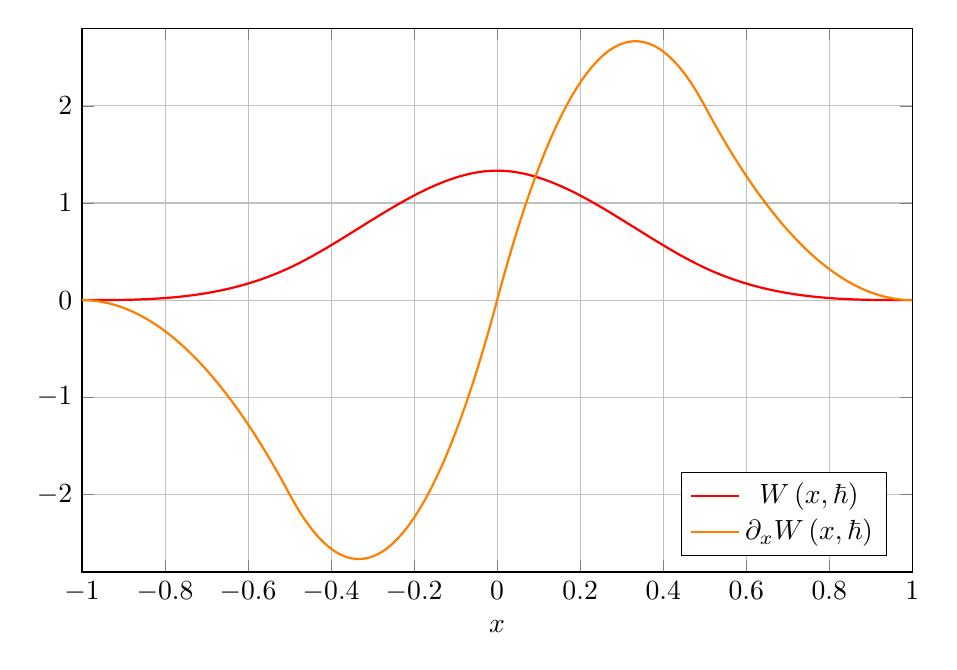
\begin{tikzpicture}[domain=0:1]
    \begin{axis}[xmin=-1, xmax=1,ymin=-2.8, ymax=2.8, grid=both,
      width=\linewidth, height=0.7\linewidth, legend pos=south east, 
      xlabel = {$x$}
      ]
      \addplot[red, thick, samples=100, smooth, domain=-1:1]  
        {8/3* (max(0,1-abs(\x))^3-4*max(0,0.5-abs(\x))^3)};
      \addplot[orange, thick, samples=100, smooth, domain=-1:1]  
        {8/3* \x / abs(\x)* (3*max(0,1-abs(\x))^2-12*max(0,0.5-abs(\x))^2)};
      \legend{$W\br{x, \hbar}$, $\partial_x W\br{x, \hbar}$}
    \end{axis}
  \end{tikzpicture}
  \caption{The $M_4$ cubic spline kernel function $W\br{x, \hbar}$ from \autoref{eq:cubic-spline} and its first derivative $\partial_x W\br{x, \hbar}$ are plotted in one dimension ($d=1, \hbar=1, \alpha_1=\sfrac{8}{3}$) for $x\in[-\hbar,\hbar]$}\label{fig:cubic-spline}
\end{figure}


Note that different kernel functions and smoothing lengths may be applied depending on the interpolated quantity and specialized, non-Gaussian-like kernel functions have been used in some scenarios \autocites{mueller-sph}{teschner-surf-tens-neg-kernel}. 

Taylor expansion of the approximation yields that the \ac{sph} method is $0^\text{th}$ and $1^\text{st}$-order accurate if all up to each of the following criteria hold \cite{tutorial2019}:
\begin{subequations}
  \label{eq:consistency-criteria}
  \begin{align}
    \sum_{j\in\mathcal{N}_i} \frac{m_j}{\rho_j} W_{ij} &= 1 &\textit{$0^\text{th}$-order accuracy}\label{eq:acc-0th-order}\\
    \sum_{j\in\mathcal{N}_i} \frac{m_j}{\rho_j} \br{\vek{x}_j - \vek{x}_i} W_{ij} &= \vek{0} &\textit{$1^\text{st}$-order accuracy}
  \end{align}
\end{subequations}


Interestingly, normalizing the kernel function such that the former holds yields the so-called Shephard-filtered field \cite{survey2022}, where the kernel is equivalent to the Shepard interpolant in the moving least squares method \cite{duarte-meshless}.
% Similarly, the latter condition can be ensured by a small matrix inversion per particle \autocites{tutorial2019}{price2012}. 
For the sake of the simplicity of both the implementation and discussion, such filtering is foregone in this report.



% In general application to SPH fluid simulation, Wendland functions and Schoenberg B-Splines (e.g. $M_4, M_6$ \cite{price2012}) are popular choices \cite{kernel-comparison-improv-convergence}, with 

% approximations to Gaussians are most widely used \cites{price2012}{kernel-comparison-improv-convergence}. 

% In this report, the classic cubic spline or $M_4$ spline with $\hbar=2h$ was chosen \cites{price2012}{sph-monaghan-92}:

\subsection{Differential Operators}
To discretize the momentum equation (\autoref{eq:momentum}), differential operators such as $\nabla, \Laplace$ must be defined on \ac{sph}-reconstructed fields. Different  gradient approximations exist, with respective benefits and drawbacks, common choices being \cite{tutorial2019}:
\begin{align}
  \abr{\nabla f_i}_{\text{direct}} &=\sum_{j\in\mathcal{N}_i} \frac{m_j}{\rho_j} f_j \nabla W_{ij} &\textit{direct}\\
  \abr{\nabla f_i}_{\text{diff}} &=\sum_{j\in\mathcal{N}_i} \frac{m_j}{\rho_j} \br{f_j - f_i} \nabla W_{ij} &\textit{difference}\\
  \abr{\nabla f_i} &= \rho_i \sum_{j\in\mathcal{N}_i} m_j \br{\frac{f_i}{\rho_i^2} + \frac{f_j}{\rho_j^2}} \nabla W_{ij} &\textit{symmetric}\label{eq:symmetric-formula}
\end{align}
The direct formula can similarly be derived for other differential operators ($\divergence, \nabla\times, \dots$) and is simple, but not preferred due to inaccuracy \cite{tutorial2019}. The difference formula compensates for the $0^\text{th}$-order error term of the gradient approximation to yield more accuracy (being exact for constant fields) and can be made exact to first order by a small matrix inversion per particle \autocites{price2012}{tutorial2019}. The symmetric formula can be derived from the discrete Lagrangian and yields symmetric pressure forces that conserve linear and angular momentum when applied to the pressure field \autocites{price2012}{tutorial2019}. While the difference formula is more asymptotically accurate at the cost of loss of momentum, the symmetric formula has superior conservation properties and results in forces that restore a preferable, uniform particle sampling, which is why it is generally preferred \cite{tutorial2019} in application to pressure gradients and was chosen in this report.


For the Laplacian of vector fields required for the computation of viscous accelerations in \autoref{eq:momentum}, a discretization must be chosen. Direct approximation of second derivatives by using $\Laplace W$ is very sensitive to the quality of the particle sampling and not robust, so it is discouraged \autocites{price2012}. A popular scheme in application to nearly divergence-free velocity fields that yields viscous accelerations which obey momentum conservation \cite{price2012} is given by:
\begin{equation}\label{eq:vis-laplactian}
  \abr{\Laplace \vek{f}_i}_\nu = 2(d+2) \sum_{j\in\mathcal{N}_i} \frac{m_j}{\rho_j}  \frac{\vek{f}_{ij} \cdot \vek{x}_{ij}}{\abss{\vek{x}_{ij}}^2+10^{-2}h^2}
\end{equation}
with regularization $10^{-2}h^2$ of the denominator. This scheme is chosen in this report for the computation of $\nu \abr{\Laplace \vek{v}}$ as often \autocite[recommended]{survey2022}.

On the other hand, for the discretization of the pressure Laplacian of the \ac{ppe} (\autoref{eq:ppe-rho-invariant}), the discretized divergence of the symmetric gradient formula is used in this report in order to ensure consistency with the computation of pressure gradients \cite{2014-survey}:
\begin{equation}
\begin{aligned}\label{eq:prs-laplacian-divergence}
  \abr{\Laplace f_i} &= \abr{\divergence \abr{\nabla f_i}}\\
  \abr{\divergence \vek{f}_i} &= -\frac{1}{\rho_i} \sum_{j\in\mathcal{N}_i} m_j \vek{f}_{ij} \cdot \nabla W_{ij}
\end{aligned}
\end{equation}

For a comparison of the discretizations of the pressure Laplacian using \autoref{eq:prs-laplacian-divergence} and \autoref{eq:vis-laplactian} see \autocite[Fürstenau et al.]{fuesrtenau-laplacian-comp}.

% Direct approximation through application to the kernel function as in $\abr{\nabla f_i} =  \sum_{j\in\mathcal{N}_i} \frac{\rho_j}{m_j} f_j \nabla W_{ij}$ (and analogous for other operators) is possible, but not preferred \autocites{tutorial2019}{liu2010}. Rather, there exist more elaborate formualtions that very by accuracy, physical conservation properties etc. 

Note that all \ac{sph}-discretizations $\abr{f}$ are linear operators in the interpolated quantities $f_i$ and commutative, e.g. for $f,g$ it holds that $\abr{f + g} = \abr{g + f} = \abr{f} + \abr{g}$ and $\abr{f  g} = \abr{g  f} = \abr{f}  \abr{g}$ \cite{liu2010}. In the same sense, $\abr{f_i}$, $\abr{\nabla f_i}$, $\abr{\Laplace f_i}$ and  $\abr{\Laplace \vek{f}_i}$ are affine functions of $[f_1, \dots, f_N]^T$ for all $i$.

\section{From Linear Systems to an Optimization Problem}
\subsection{Setting}
Using the governing equations as well as their discretization in time and space outlined in the previous sections, the setting of the optimization problem can precisely be formulated. 

In the absence of vorticity models and other modifications \autocite{tutorial2019}, the state of the fluid at each point in time $t$ can uniquely be described using only the set of all $N$ particle positions and velocities, so the state space is comprised by:
\begin{align}
  \mat{X} &:= \left[\vek{x}_1, \dots, \vek{x}_N\right]\\
  \mat{V} &:= \left[\vek{v}_1, \dots, \vek{v}_N\right]
\end{align}
Parameters that are constant throughout the simulation, which is conducted in two dimensions ($d=2$), include:
\begin{itemize}
\item time step size $\Delta t$ $[\text{s}]$ (see \autoref{sec:time-discretization})
\item acceleration due to gravity $\vek{g}$ $[\frac{\text{m}}{\text{s}^2}]$
\item kinematic viscosity $\nu$ $[\frac{\text{m}^2}{\text{s}}]$
\item rest density $\rho_0$ $[\frac{\text{kg}}{\text{m}^2}]$
\item particle mass $m$ $[\text{kg}]$ (here: $\forall i,j\in\mathds{N}_1^N: m_i = m_j = m$)
\end{itemize}

The decision variables of the problem of \ac{sph} pressure computation for incompressible fluids is one scalar pressure value per particle (since directions of symmetric pressure gradients follow from the particle positions $\mat{X}$ by \autoref{eq:symmetric-formula} as to conserve linear and angular momentum):
\begin{equation}
  \vek{p} = \left[ p_1, \dots, p_N \right]^T
\end{equation}

These pressure values are defined to satisfy the continuity equation (\autoref{eq:continuity}) for incompressible fluids, yielding the \acf{ppe} in \autoref{eq:ppe-rho-invariant}:
\begin{equation}
  \Delta t^2 \Laplace p_i = \rho_0 - \rho^*(t+\Delta t)
\end{equation}
where the right side of the equation is the linearized, density-invariant incompressibility constraint derived from \autoref{eq:source-rho-abs}. This term can be discretized in space using \ac{sph} interpolation as described in \autoref{sec:sph} and operator splitting with intermediate velocities $\vek{v}^*$ from symplectic Euler as described in \autoref{sec:time-discretization} can be applied, resulting in:
\begin{align}
  &\Delta t^2 \abr{\divergence \abr{\nabla p_i}} \\
  &= \rho_0 - \abr{\rho_i} + \Delta t \abr{\rho_i}\abr{\divergence \vek{v}^*_i}\qquad\textit{by \autoref{eq:rho-change-non-pr}}\\
  &= \underbrace{\rho_0 - \abr{\rho_i} + \Delta t \abr{\rho_i}\abr{\divergence \br{\vek{v}_i + \Delta t \vek{g} + \Delta t \abr{\nu\Laplace\vek{v}_i}}}}_{s_i :=}  % = \abr{\rho_i} + \Delta t \abr{\frac{D\rho_i}{Dt}}
  \label{eq:ppe-sph-discretized}
\end{align}
Note that the source term $s_i$ in \autoref{eq:ppe-sph-discretized} is known ($\vek{v}_i$ from $\mat{V}$, $\vek{g}$ is constant, $\abr{\rho_i}$ is a function of $\mat{X}$ and $m$ via \autoref{eq:density-estimate} and will therefore synonymously be denoted $\rho_i$) while the left is a change in density due to unknown pressure accelerations.

Given a valid set of pressure values, accelerations are then computed by the \ac{sph}-discretization of the momentum equation (\autoref{eq:momentum}):
\begin{equation}\label{eq:discretized-momentum}
  \abr{\vek{a}_i }= -\frac{1}{\abr{\rho_i}}\abr{\nabla p_i} + \abr{ \nu \Laplace \vek{v}_i} + \vek{g}
\end{equation}

Finally, the kinematics of the system follow the \acs{ode} in \autoref{eq:eqs-of-motions}:
\begin{align}
  \dot{\vek{v}} &= \vek{a}\\
  \dot{\vek{x}} &= \vek{v}
\end{align}
which for a discrete time setting using symplectic Euler integration as discussed in \autoref{sec:time-discretization} means, as in \autoref{eq:semi-implicit-euelr}:
\begin{align}
  \vek{v}\br{t + \Delta t} &= \vek{v}(t) + \Delta t \vek{a}(t)\\
  \vek{x}\br{t + \Delta t} &= \vek{x}(t) + \Delta t \vek{v}\br{t + \Delta t}
\end{align}
and updates the system state $[\mat{X}, \mat{V}]$ from some time $t$ to the subsequent time step $t+\Delta t$. 

A desired initial state of a fluid at some time $t_0$ at rest is typically sampled on a regular grid of spacing $h$ (which defines the constant kernel support radius $\hbar=2h$) to obtain $[\mat{X}, \mat{V}](t_0)$.

To finalize the mixed initial-boundary value problem, boundary conditions are incorporated. In the simplest case, this can be done by sampling the boundary in $\lceil \sfrac{\hbar}{h} \rceil+1 = 3$ layers (as to fill the kernel support radius at the boundary) on the same regular grid of spacing $h$ and with the same mass $m$ as the fluid particles, except boundary particles have fixed positions in time. Single layer, non-uniform sampling could be implemented by adjusting the masses of boundary particles \cite{boundary2012akinci}. Contact forces are then naturally handled as pressure forces by extending all \ac{sph} sums to include boundary particle positions in some static $\mat{X}_b$ with mass $m$, with no other changes to the system required. Instead of extending the \ac{ppe} to include boundary particles explicitly \cite{pressure-boundaries}, mirror \cite{boundary2012akinci} or extrapolate pressure values \cite{mls-extrapolated-pressure-boundaries}, this report opts to use \textit{consistent boundaries} by asserting $p=0$ at boundary particles, improving stability and simplicity of the formulation \autocites{consistent-boundaries}{unified-pressure-probst}.


% To finalize the mixed initial-boundary value problem of computing particle trajectories over time in a desired scene, an initial state $[\mat{X}, \mat{V}](t_0)$ at some time $t_0$ is given; typically by sampling the desired fluid at rest density on a regular grid of spacing $h$ (defining the kernel support radius $\hbar=2h$). Boundary conditions are here chosen to be implemented monolithically in the exact same way as fluid particles, except they are static in time, i.e. $\frac{D\vek{x}}{Dt} = \vek{0}$, sampled in $\lceil \sfrac{\hbar}{h} \rceil+1 = 3$ layers on a uniform grid, such that boundary particles can fill the kernel support of non-penetrating fluid particles, and exhibiting $p_i=0$ for all $i$ in the boundary. This means that contact forces are handled as pressure forces and no further distinction between fluid and boundary particles must be made, which will not be considered in any .

\subsection{Free Surface Effects}\label{sec:free-surface-effects}
So far, pressure computation in every time step is formulated as a system of $N$ equations in \autoref{eq:ppe-sph-discretized}. Since all chosen SPH-discretizations $\abr{\cdot}$ on some field $f$ are linear functions of the sampled quantities $[f_1,\dots,f_N]^T$ at particle locations $\mat{X}=[\vek{x}_1,\dots,\vek{x}_N]$ that they are interpolating, the pressure Laplacian $\abr{\Laplace p_i} = \abr{\divergence \abr{\nabla p_i}}$ in particular and therefore the discretized \ac{ppe} is simply a linear system of equations in unknown pressure values $p_1, \dots, p_N$. 



% This could be interpreted as the unconstrained minimization of the quadratic form the minimizer of which solves the linear system, where pressures are e.g.:
% \begin{equation}
%   \argmin_{p_1,\dots,p_N} \sum_{i=1}^{N} \br{\abr{\divergence \abr{\nabla p_i}} - \frac{s_i}{\Delta t^2}}^2
% \end{equation}
% and the minimum is at zero.


% This means that for given particle positions $\mat{X}$, resulting densities $\abr{\rho_i}$ and particle mass $m$ there exist linear maps (or tensors) $\mat{G}, \mat{L}$ that implement the \ac{sph}-discretized gradient and Laplace-operators, respectively. 

There are two issues with this formulation that result directly from the \ac{sph} method, one of which (negative pressure values) is commonly addressed in practice and the second of which (density underestimation) will lead to the objective function of the optimization problem formulated in this report. Both of these defects can be illustrated by the behaviour of the fluid at the free surface. 

In order to reconstruct a valid approximation of underlying field quantities, \ac{sph} sums over quantities sampled at neighbouring particle locations within the kernel support radius $\hbar$. At the free surface, this approximation becomes inaccurate due to \textit{particle deficiency} \cite{tutorial2019}, since only part of the support domain is sampled. This is easily confirmed by considering the criteria for consistency of the approximation in \autoref{eq:consistency-criteria}: at the surface, $0^\text{th}$-order accuracy is clearly violated, since \cite{liu2010}:
\begin{equation}
  \sum_{j\in\mathcal{N}_i} \frac{m_j}{\rho_j} W\br{\vek{x}_i-
  \vek{x}_j, \hbar} < 1
\end{equation} 
which means that even a constant field cannot be accurately reconstructed due to lack of neighbours in $\mathcal{N}_i$ for $i$ at the free surface. In other words, the collocation to particle positions leads to inaccuracies at the free surface since the interpolants do not form a partition of unity, as demanded by \autoref{eq:acc-0th-order}. Another intuition is that since the smoothing kernel is not truncated at the fluid domain's boundary but extends past it, and it is normalized across its entire support domain, the free surface that can be thought of as a discontinuity in the mass field is smoothed in space much in the same way that all other field quantities are, leading to a biased estimate. 

Looking at the basic \ac{sph} interpolation in \autoref{eq:sph-sum-basic} as a sum over neighbouring particles, a lack of such neighbours is equivalent to a sampling of the field with a value that corresponds to the neutral element of that sum: positive scalar fields are underestimated since points outside the fluid assume the value $0$, negative fields are analogously overestimated, estimates of vector fields are skewed towards $\vek{0}$ in the direction of missing contributions etc. 

This means that there are implicit boundary conditions that so far have not been made explicit: pressures and densities outside the fluid take on the value zero. Both of these effects have direct consequences on the simulation and can be corrected using inequality constraints, which are discussed in order in the following.

\section{Modelling Constraints}
\subsection{Pressure Positivity}
Ideally, shifting the entire pressure field by a constant offset should not influence the resulting pressure gradient field. In \ac{sph} however, a pressure gradient despite a constant pressure field is induced at free surfaces (and to some extent in all regions with unfortunate particle configurations) where the pressure field differs from its implicitly assumed value in the absence of samples, namely zero. Since consistent boundaries \cite{consistent-boundaries} with $p=0$ were chosen in the implementation of solid boundary conditions, solid boundaries behave much the same as the free surface in this regard. Therefore, the pressure that is computed by the \ac{ppe} should certainly be non-negative in order to avoid spurious pressure gradients at the boundary, yielding an inequality constraint:
\equationnamed{Pressure Positivity}{
  \begin{equation}\label{eq:pressure-positive}
    \forall i\in\mathds{N}_1^N: \quad p_i \geq 0 
  \end{equation}
}
This is a more formal interpretation of what practitioners already do: \ac{iisph} \cite{iisph} suggests that while solving the \ac{ppe} using a relaxed Jacobi scheme for example, all pressure iterates should simply be clamped to non-negative values, resulting in a projected Jacobi scheme, referencing how equation-of-state based solver similarly clamp negative pressures to avoid excessive attractive pressure forces where predicted densities fall below rest density \cite{iisph}. \autocite[Other authors]{tutorial2019} similarly suggest pressure clamping in reference to the implicitly zero pressure in the absence of particles. In this report, the same suggestion is not an implementation recommendation but formalized as an inequality constraint on the permissible set of solutions.

\subsection{Compression and Density Deviation}
Another related implicit constraint due to particle deficiency can be observed that is already handled, albeit perhaps difficult to spot, by many popular \ac{sph} schemes in implementation. In the same way that pressures are implicitly zero outside the fluid domain, so is the volumetric mass density. 

This leads to the problem that if $\rho\br{t+\Delta}=\rho_0$ is enforced, particles at the free surface that famously \cite{tutorial2019} suffer from an underestimation of the density field by the \ac{sph}-approximation in \autoref{eq:density-estimate} due to neighbour deficiency and must compensate for this lack of contributions in the kernel support domain by clustering together in order to achieve rest density, leading to clumping artefacts at the surface that manifests similarly to an excessive surface tension \cite{iisph}. The discretized \ac{ppe} was previously mentioned to be a linear system due to \ac{sph}-approximations being linear operators on sampled fields, which means that the \ac{sph}-discretized \ac{ppe} can be written in some form:
\begin{equation}
  \mat{L}\vek{p} = \vek{s}
\end{equation}
where $\vek{p}\in\mathds{R}^N$ are all pressure values, $\vek{s}\in\mathds{R}^N$ is a collection of source terms $s_i$ scaled by $\frac{1}{\Delta t^2}$ (see \autoref{eq:ppe-sph-discretized}) and $\mat{L}\in\mathds{R}^{N\times N}$ represents a discrete Laplacian operator that depends on particle positions $\mat{X}$ as well as densities derived from it through constant particle masses by \autoref{eq:density-estimate}. Note however that $\mat{L}$ is generally only positive semidefinite, meaning that a unique solution to this system of equations might not exist. This becomes obvious considering the effect of density underestimation on isolated particles: a fluid particle with no neighbours will estimate its own density due to \autoref{eq:density-estimate} to $m \cdot W(\vek{0}, \hbar)$ and have absolutely no way of compensating for deviation from $\rho_0$, irrespective of pressure values (which are arbitrary anyway, because pressure gradients at isolated particles are always zero, since $\nabla W_{ii}=\vek{0}$ due to symmetry and continuity of $W$ demanded in \autoref{eq:kernel-criteria}). If the isolated particle were in the vicinity of boundary particles, unintended sticking artefacts and non-separating boundary conditions would result from the pressure forces compensating for the underestimated density by more closely approaching the boundary particles. More generally, density is underestimated not just at isolated particles, but along the entire free surface, exasperating the problem. 

One way to reformulate the problem as to avoid this artefact of the discretization is to demand that not all deviations from rest density, but only positive deviations or compressions be penalized by the source term. This would mean that instead of a linear equality constraint on pressures imposed by the \ac{ppe} in \autoref{eq:ppe-sph-discretized}, one would instead incorporate an incompressibility constraint through an inequality:
\equationnamed{Positive Incompressibility}{
  \begin{align}
    \Delta t^2 \Laplace p_i + \rho_i^*(t+\Delta t) &\leq \rho_0 \\
    % \underbrace{
      \abr{\rho_i} \underbrace{ - \Delta t \abr{\rho_i}\abr{\divergence \vek{v}^*_i}}_{\abr{\Delta \rho_i}_{\nu,g}}  + \underbrace{\Delta t^2 \abr{\divergence \abr{\nabla p_i}}}_{\abr{\Delta \rho_i}\br{\vek{p}}}
    % }_{\abr{\rho_i^{**}}(\vek{p}) :=}
    &\leq \rho_0\label{eq:incompressibility-positive}
  \end{align}
}

The updated predicted density on the left side of this inequality, which includes changes in density due to pressures $\abr{\Delta \rho_i}\br{\vek{p}}$, will be named $\abr{\rho_i^{**}}(\vek{p})$. One disadvantage of this reformulation is that suction, in the sense of pressure gradients induced by a density below $\rho_0$ \textit{within} the fluid domain are also disabled, not just at the free surface, meaning that for example tight vortices in low-viscosity flows can cause gaps in the particle sampling to form as particles spiral outwards from the vortex's centre with no pressure forces to close the forming 'vacuum' of particles. 

This trade-off seems to be accepted in practice, since many pressure solvers, despite not explicitly claiming to do so, seem to actually implement this inequality constraint in some form. It could be argued that in \autocite[\ac{iisph}]{iisph} for example, operator splitting leads to predicted velocities that tend to represent a compressed state, for example due to gravity accelerating fluid particles towards a solid boundary, resulting in a predicted density above $\rho_0$. This positive compression is then minimized by iteratively determining positive pressure values that compensate for density deviations, but crucially, pressures are often initialized to zero (meaning that pressure gradients are as well), density deviation due to pressures $\abr{\Delta \rho_i}_{p}$ is a linear function of said pressure gradients and the convergence criterion of the pressure solver minimizing the total density deviations is defined in iteration $k$ as an inequality:
\begin{equation}\label{eq:iisph-termination}
  \br{\frac{1}{N}\sum_{i=1}^N \abr{\rho_i^{**}}(\vek{p})} - \rho_0 < \epsilon
\end{equation} 
for some threshold $\epsilon$ on the order of $10^{-3}\rho_0$ \cite{iisph}. This means that if predicted density is below rest density, the solver terminates after a set minimum amount of iterations, irrespective of the deviation between each predicted density and rest density. If on the other hand compressions are positive to begin with and the predicted density decreases throughout each iteration, then due to the termination criterion, negative divergence of pressure gradients grows until an approximation of $\rho\br{t+\Delta t} \leq \rho_0$ is effectively enforced, not strictly $\rho\br{t+\Delta t} = \rho_0$. 

In a similar vein, \autocite[\ac{dfsph}]{dfsph} uses a source term based on the divergence-free constraint in \autoref{eq:source-div-free} in its respectively named sub-solver, says to compute $\frac{D\rho}{Dt}=-\rho_i\divergence\vek{v}_i^*$ and from it, derive pressure gradients that project the predicted velocity field due to non-pressure accelerations $\vek{v}^*$ onto a divergence-free state \cite{dfsph}. The implementation of the solver named \autocite[SPlisHSPlasH]{SPlisHSPlasH_Library}, by the same authors, does \textit{not} compute this quantity but instead clamps it to non-negative values, i.e. $\frac{D\rho}{Dt}'=\max\br{0, -\rho_i\divergence\vek{v}_i^*}$ and therefore only penalizes positive compressions, effectively enforcing \autoref{eq:incompressibility-positive}. Furthermore, the same implementation completely disables the divergence-free source term by setting $\rho_i^*(t+\Delta t) = \rho_0$ at the free surface through a heuristic that compares the cardinality of the neighbour set $\abs{\mathcal{N}_i}$ to user-defined values such as $7$ in 2D and $20$ in 3D, relying only on the density-invariant source term when a particle is suspected to be at a free surface, thereby avoiding the conceptual issue in a rather ad-hoc way.


While the explicit, inequality-based formulation of \autoref{eq:incompressibility-positive} indeed represents a trade-off between the artefacts that it avoids and others that it causes, both of which arise due to inherent inadequacies of the \ac{sph} method, this report would like to argue that the inequality-based formulation is, in fact, what people deem more accurate and implement in practice, despite deriving the computation from an equality-based \ac{ppe}. One core observation in this project is that in actuality, practitioners seem to not be solving a linear system of equations but an ill-posed optimization problem that can be improved by introducing a physically meaningful objective function, such as the one suggested in \autoref{sec:pmpg}.



\subsection{Defects of Current Methods and Ill-Posed Optimizations}

% Assuming that the claim that existing methods in fact minimize some measure of the predicted density $\abr{\rho_i^{**}}(\vek{p})$ in \autoref{eq:incompressibility-positive} subject to pressure positivity (\autoref{eq:pressure-positive}) holds, some surprising and unintended behaviours of existing solvers can be explained by analysing the implemented optimization problem.

The problem of minimizing the upwards-constrained, left side of the termination criterion of the \ac{iisph} solver in \autoref{eq:iisph-termination}, subject to $\vek{p}\geq 0$, would be:
\begin{equation}\label{eq:ill-posed-problem}
  \begin{aligned}
    &\min_{\vek{p}\in\mathds{R}^N} & \frac{1}{N}\sum_{i=1}^{N}
      \abr{\rho_i^*} + \Delta t^2 \br{\mat{L}\vek{p}}_i -\rho_0 \\
    &\text{s.t.} & \vek{p} \geq 0
  \end{aligned}
\end{equation}

where $\mat{L}(\mat{X},m)\in\mathds{R}^{N\times N}$ is the positive semidefinite \ac{sph}-discretized Laplacian operator for given particle masses and positions. In this \ac{lp} there is no dependence of $\abr{\rho_i^*}$ and $\rho_0$ on $\vek{p}$, so the constant terms can be neglected, meaning that positivity of pressures defines a half-space of feasible pressure values $\Omega = \left\{\vek{p}\in\mathds{R}^N \,\middle|\, \vek{p}\geq 0 \right\}$ and the level sets of the objective function are parallel hyperplanes. From this geometry it follows that unless such hyperplanes all have a non-negative derivatives in all dimensions such that $\vek{p}=\vek{0}$ becomes a minimizer, the objective is unbounded below, the problem is ill-posed and no minimum exists. This also makes intuitive sense, since for any particle configuration with a non-empty edge set of the connectivity graph, positive pressure values can always be chosen that result in pressure gradients with arbitrary divergence. In other words, one may always choose positive pressures such that the liquid explodes, trivially resulting in an uncompressed state. Clearly, this is unintended.


However, a solver attempting to iteratively solve the above, ill-posed optimization problem can indeed be used to solve the related problem of finding any positive pressures $\vek{p}\geq \vek{0}$ that result in an uncompressed state. Considering from now on both inequalities (\autoref{eq:pressure-positive}, \autoref{eq:incompressibility-positive}) to be inequality constraints, they form a feasible set that is the intersection of a half-space ($\vek{p}\geq \vek{0}$) and the level set of a hyperplane in the space of pressures. If this feasible set:
\begin{equation}\label{eq:feasible-pressures}
  \Omega = \left\{\vek{p}\in\mathds{R}^N \,\middle|\, \vek{p}\geq 0 \land \frac{1}{N}\sum_{i=1}^{N}
  \abr{\rho_i^*} + \Delta t^2 \br{\mat{L}\vek{p}}_i -\rho_0 < \epsilon \right\}
\end{equation} 
is not empty, then an iterative solver respecting the former inequality while minimizing the upwards-constrained side of the latter might at some point find a first iterate $\vek{p}^{[k]}$ in some iteration $k$ that lies in $\Omega$. It could be argued that this is what commonly used \ac{sph}-based pressure solvers actually do: they find some first feasible point in a convex polytope, or a first uncompressed state in the space of pressure vectors, by abusing solvers for linear systems. 

Crucially, this is not truly an optimization problem since it lacks an objective function, which is to be fixed in \autoref{sec:pmpg}. The first feasible point is therefore not the least feasible point in any intuitive sense, but rather an implementation-dependent and therefore arbitrary feasible point, and as previously mentioned explosions of the fluid are unfortunately feasible. If this model of how pressure solvers can be thought to behave in implementation is accurate, it would explain otherwise surprising behaviour well:
\begin{itemize}
  \item Projected, Relaxed Jacobi-based \ac{iisph} pressure solvers can be sensitive to initialization. Despite the obvious improvement offered by warm-starting the solver by initializing it to the pressures calculated in the previous time step and exploiting how similar subsequent pressure computation problems are, especially for small $\Delta t$, this is surprisingly not done in practice since it might incur instabilities of the solver that manifest as explosions. Such problems can even be inherited to an extent by more elaborate pressure solvers such as the \ac{nncg} method applied by \autocite[Probst and Teschner]{unified-pressure-probst} to the problem of \ac{sph} pressure computation formulated as a \ac{lcp} per time step and using a Jacobi-based sub-solver inside a Fletcher-Reeves-type \ac{cg} method.
\end{itemize}

It could be speculated that this behaviour is also part of the reason why \textit{smoother} solvers such as relaxed Jacobi, which monotonously decrease every eigenvector component of the residual in each iteration \cite{painless-cg}, appear to be more stable in practice, especially when cold-started to $\vek{p}=\vek{0}$ \cite{iisph}, while \textit{rougher} solvers such as Steepest Descent and \ac{cg} \cite{painless-cg} are found to be more unstable and behave erratically \cite{iisph}: since \autoref{eq:incompressibility-positive} is actually enforced and the set of feasible pressure gradients is upwards unbound with no objective function to prevent explosions, smoothing solvers just happen to tend to find a \textit{first} feasible iterate that is closer to the optimal, \textit{least} feasible iterate, which is actually desired. In other words, conservatively initialized smoothing solvers do not tend to overshoot the ideal pressure gradient field as much when searching for any $\vek{p}\in\Omega$.

This would mean that nothing about the problem statement guarantees a solution, let alone a least or even unique least solution, and more stable, cold-started solvers just happen to be implemented in such a way that pressures close to the optimal pressure field are often found. Clearly, a physically motivated objective function that defines a least pressure within the set $\Omega$ (\autoref{eq:feasible-pressures}) of feasible pressures and yields a well-posed optimization problem would be more ideal. Finding such a function is the subject of \autoref{sec:pmpg}.


\section{Designing an Objective Function}\label{sec:pmpg}
A few objective functions and approaches were considered in the process of trying to define the least vector of positive pressures that yields an uncompressed predicted \ac{sph} fluid state at the next time step. Some resulting ideas that did not bear fruit included the following:
\begin{itemize}
  \item An exact penalty method was considered, where the constraint $\vek{p}\geq 0$ is enforced but a regularization term of the form $\alpha \abss{\vek{p}}_\ell$ for a small $\alpha$ and some $\ell$-norm is added to the objective function of \autoref{eq:ill-posed-problem}. The choice of $\alpha$ would create an unintuitive and scene-dependent parameter that appears hard to estimate reasonable values for. Furthermore, minimizers would differ slightly depending on this value of $\alpha$, which is not ideal.
  \item A lexicographic optimization was considered, where compression is first minimized subject to pressure positivity, then pressures are minimized. While this sounds logical, the first stage of this problem is not well-posed for the same reasons as for \autoref{eq:ill-posed-problem}, and even then, since the ideal compression is known to be zero, the first stage becomes unnecessary and the second stage could be conducted right away, leading to the next idea:
  \item A simple, inequality-constrained optimization was considered, where \autoref{eq:pressure-positive} and \autoref{eq:incompressibility-positive} serve as inequality constraints while some $\ell$-norm of $\vek{p}$ is minimized. This could be implemented as a \ac{lp} for $\ell=1$ or $\ell=\infty$ or a \ac{qp} for $\ell=2$. While this is close to what is actually done in \autoref{sec:least-pressure-gradient}, the choice of $\ell$ and interpretability of this choice remained an open question.
  \item Minimization of a \ac{ncp} function such as the Fischer-Burmeister function \cite{burmeister-idee} $a+b-\sqrt{a^2+b^2}$ was considered \cite{fisher-burmeister}, where $a$ could be pressure and $b$ could be compression, similar to the \ac{lcp} approach by \autocite[Probst and Teschner]{unified-pressure-probst}. It is not immediately obvious how pressures and compressions with differing units are best summed, if they should be made dimensionless with respect to some characteristic quantities or related to one another by an equation of state for example, as well as why complementarity of pressure and compression should necessarily be demanded and how the resulting optimization is best implemented.
\end{itemize}

The final objective function was found thanks to the work of \autocite[Alhussein and Daqaq]{pmpg} who, based on Gau\ss's principle of least constraint, propose to minimize the physical action of gradient fields that give rise to constraint forces, subject to their constituting constraints, and use this to conduct physics-informed machine learning. This results in a physically meaningful, interpretable and easy to implement objective function in this context, which yields one convex \ac{qp} to solve per time step.

\subsection{Principle of Least Constraint}\label{sec:least-pressure-gradient}
The objective function that was chosen in this report is based on the \emph{Principle of Least Constraint}, formulated by \autocite[Carl Friedrich Gau\ss]{Gauss-least-action} and which states that in any instance in time, a system of $N$ point masses of masses moving under a constraint will move in the greatest possible accordance with their unconstrained, free movement - or with the least constraint - in the sense that a sum of the mass-weighted squares of the deviation between the position after some infinitesimal time step $dt$ in the constrained and unconstrained case be a minimum \cite{Gauss-least-action}. This can be written as the minimum of the \emph{action} $S$ \cite{pmpg}:
\begin{align}
  S &=\frac{1}{2} \sum_{i=1}^{N} m_i \br{\vek{a}_i - \frac{\vek{F}_i}{m_i}}^2\\
  &= \frac{1}{2} \sum_{i=1}^{N} \br{\frac{\vek{R}_i}{m_i}}^2
\end{align}
where $\vek{F}_i = m\vek{a}_i - \vek{R}_i$ are external forces and $\vek{R}_i$ are constraint forces \cite{pmpg}. Using the fact that we choose constant particle masses $m_i = m$ and that pressure is the constraint force in this scenario, the $i$-th acceleration $\frac{\vek{R}_i}{m_i}$ due to pressure forces follows from the momentum equation (\autoref{eq:momentum}, \ac{sph}-discretized to \autoref{eq:discretized-momentum}) and reads $-\frac{1}{\rho_i} \abr{\nabla p_i}$. Since in any time step, positions $\mat{X}$, masses $m$ and therefore densities $\rho_i$ from \autoref{eq:density-estimate} as well as the factor $\frac{1}{2}$ can be considered constant, a function $S: \mathds{R}^N \to \mathds{R}_+$ of unknown pressures $\vek{p}$ proportional to the action can be defined simply as:

\begin{align}
  S(\vek{p})
  &= \sum_{i=1}^{N} \abr{\nabla p_i}^2 &\\
  &= \sum_{i=1}^{N} \br{\rho_i \sum_{j\in\mathcal{N}_i} m_j \br{\frac{p_i}{\rho_i^2} + \frac{p_j}{\rho_j^2}} \nabla W_{ij}}^2& \textit{\autoref{eq:symmetric-formula}}\\
  % &\propto \sum_{i=1}^{N} \br{\sum_{j\in\mathcal{N}_i} \br{\frac{p_i}{\rho_i^2} + \frac{p_j}{\rho_j^2}} \nabla W_{ij}}^2 &
\end{align}
where $\nabla W_{ij}$ (\autoref{eq:cubic-spline}) and $\mathcal{N}_i$ (\autoref{eq:neighbour-set-def}) depend on the particle configuration $\mat{X}$. 

\section{Optimal Incompressible \ac{sph} Pressure Fields}

Denoting the symmetric, \ac{sph}-discretized gradient operator in \autoref{eq:symmetric-formula} as $\mat{G}\in\mathds{R}^{N\times N}$, one can see that:
\begin{align}
  S(\vek{p}) = \br{\mat{G}\vek{p}}^2 
  = \br{\mat{G}\vek{p}}^T \br{\mat{G}\vek{p}}
  = \vek{p}^T\br{\mat{G}^T \mat{G}}\vek{p}
\end{align}
and since real-valued Gram-matrices of the form $\mat{G}^T \mat{G}$ are always symmetric and positive semidefinite, so are the Jacobian and the constant Hessian of $S$ with respect to $\vek{p}$, meaning that $S$ is a convex quadratic function in $\vek{p}$. Since the feasible set $\Omega$ in \autoref{eq:feasible-pressures} is a convex set, minimizing $S$ over all $\vek{p}\in\Omega$ yields a convex \ac{qp} with a least-squares objective in each time step. This yields the optimization problem for optimal \ac{sph}-discretized pressure fields for incompressible flow that is the main result of this report:

\equationnamedbox{The Incompressible \ac{sph} pressure \ac{qp}}{
  \begin{equation}\label{eq:incompressible-qp}
    \begin{aligned}
      &\min_{\vek{p}\in\mathds{R}^N} &S\br{\vek{p}} &= \sum_{i=1}^{N}\abr{\nabla p_i}^2\\
      &\quad\text{s.t.} & \vek{p} &\geq 0\\
      &\forall i\in\mathds{N}_1^N: & \rho_0 &\geq \Delta t^2 \abr{\Laplace p_i} + \rho_i^*(t+\Delta t) 
    \end{aligned}
  \end{equation}
}
where both inequality constraints are affine functions in $\vek{p}$.

We minimize action to obtain a physically valid result, subject to the incompressibility formulated as an inequality constraint instead of an equality, in order to avoid clumping artefacts due to particle deficiency at the free surface, and subject to pressure positivity as an inequality constraint, in order to combat spurious pressure gradients at the boundary.



The resulting optimization problem is convex, therefore yielding a unique minimum $S^*\br{\vek{p}^*}$, although uniqueness of the minimizer $\vek{p}^*$ would require showing for example that $S$ is strictly convex. This is not the case in general, since any particle configuration with an isolated particle $i$ and therefore $\forall p_i \in\mathds{R}: \abr{\nabla p_i}^2 = 0$ clearly lies in the null-space. It is apparent that such null-space ridges in the objective function caused by isolated particles can be:
\begin{enumerate}
  \item detected, since if particle $i$ is isolated, then ${\nabla p_i}^2 = 0$ and the $i$-th summand of the objective function at any minimizer $\vek{p}^*$ will be zero, while the neighbour set $\mathcal{N}_i=\emptyset$ is empty
  \item fixed, since if such a particle can be detected and results in pressures being arbitrary, the smallest feasible pressure $p_i=0$ can be assigned to obtain another minimizer $\vek{p}^*\prime$ that does not suffer from the same ambiguity of $p_i$, eliminating one component of the null-space by effectively removing one degree of freedom from the system.
\end{enumerate}

It is less than obvious if this is sufficient to show that some $S\prime$ can be constructed that is positive definite and yields a unique pressure field. Note that only pressure gradients, not pressures, are relevant to the trajectories of the particles in \autoref{eq:discretized-momentum}, meaning that unique pressure gradients are perhaps as desirable as unique pressures, which are relevant only in some contexts. Boundary conditions with $p=0$ explicitly at solid boundaries by using \autocite[consistent boundaries]{consistent-boundaries} as well as an implicit $p=0$ at free surfaces due to particle deficiency suggests that zero-modes that might appear if a constant pressure field is feasible for a connected component of particles in the connectivity graph, might in fact be unique here due to the boundary conditions forcing that constant pressure to be zero, lest a pressure gradient at the boundary would follow that increases the objective function. 
Other, more exotic zero-modes that might be caused by a perfectly symmetric particle configuration causing $\sum_{j\in\mathcal{N}_i} m_j\nabla W_{ij}$ to be exactly zero are unlikely to occur in practice. 
A computationally feasible procedure for choosing a unique minimizer from the set of minimizers of \autoref{eq:incompressible-qp} that can be rigorously proven to represent the unique minimum of a positive definite action function $S\prime$ remains elusive for now and should be investigated.


Note that the gradient operator $\mat{G}$ and the Laplacian operator $\mat{L}$ defining the feasible set in \autoref{eq:feasible-pressures} share the same sparsity pattern that depends on the connectivity graph of particles within one another's kernel support radius $\hbar$, which could be abused for the efficiency of the implementation. 


Furthermore, and crucially since this was a major design goal in formulating the optimization problem, since the least feasible pressures are found and appear to be unique up to either fixable (isolated particles) or unlikely (other zero-modes) scenarios, the dynamics resulting from the pressure gradients should be invariant to the specifics of the solver implementation and the initialization of the solver, unlike some existing \ac{sph}-pressure solvers that can become unstable if initialized too far from $\vek{p}=\vek{0}$. This is one of the main motivations behind this formulation, since it would allow the similarity of pressure computation problems in subsequent time steps to be exploited by aggressively warm-starting the solver (e.g. $\vek{p}^{[0]}(t) = \vek{p}^*(t-\Delta t)$) and could open the door to heuristics-based initialization of the pressure solver based for example on known hydrostatic pressures in the steady state, if such solutions are known a priori, leaving only dynamic pressures to be computed by the solver. This would ideally result in many time steps where overall solver convergence is close to local convergence to the solution, cutting the required iteration count down and improving computational efficiency. A robust scheme for eliminating the null-space of the least-squares objective function $S$ is therefore very desirable.

Finally, note that the scale of the resulting optimization problem is exceedingly large in practice, where $N$ can easily be on the order of millions, which basically necessitates a massively parallel, GPU-based implementation and extensive abuse of sparsity patterns. To extend the following proof of concept that comprises only hundreds of particles and focuses on optimality rather than performance, computed using a CPU-based \ac{ipm} solver, to practically relevant scenarios, a parallel solver implementation for \ac{qps} that can handle sparse quadratic objectives and sparse, affine inequality constraints would be required, which seems untrivial.

\section{Results}\label{sec:results}
The \ac{qp} in \autoref{eq:incompressible-qp} was implemented in the Python programming language with the symbolic framework \autocite[CasADi]{casadi} using the \textit{Opti stack} to specify the \ac{qp} and solve it using the \ac{ipm} solver \autocite[IPOPT]{ipopt}. Due to the focus on this report on correctness and optimality rather than performance, the flexibility offered by an \ac{ipm} solver was preferred over a possibly more efficient, specialized \ac{qp} solver, especially since the prototyping phase of the project included experimentation with non-linear objective and constraint functions (see \autoref{sec:nlp-attempt}). The \textit{Opti stack} made it simple to verify that sections of code were working consistently across conventional and optimization-based pressure solvers by allowing many of the same or similar functions to either manipulate the fluid state for conventional solvers or a symbolic variable for the optimization-based approach. The optimization problem was reformulated in every time step due to changing sparsity structure of the underlying functions caused by particle movements, invalidating the results obtained by automatic differentiation offered by CasADi - this should be improved upon in the future for efficiency.

\subsection{Comparison to Predictive-Corrective Incompressible SPH}
The \ac{qp}-based pressure solver from \autoref{eq:incompressible-qp} was compared to a conventional, incompressible \ac{sph} pressure solver called \acf{pcisph}, which is simple to implement but can be shown to be essentially equivalent \cite{survey2022} to most popular \ac{sph} pressure solvers such as \autocite[\ac{pbf}]{pbf}, \autocite[\ac{iisph}]{iisph} and \autocite[\ac{dfsph}]{dfsph}.

\ac{pcisph} essentially just uses operator splitting to obtain predicted densities from predicted velocities due to non-pressure accelerations, as in \autoref{eq:rho-change-non-pr}, then relates these densities to pressures using an equation of state, namely the ideal gas equation $\Delta p = \delta \br{\rho_i^*(t+\Delta t) - \rho_0}$ with a specialized, geometrically motivated stiffness constant $\delta$ \cite{pcisph}:
\begin{equation}
  \delta = -\br{
    \Delta t^2m^2\frac{2}{\rho_0^2} \br{
      -\br{\sum_{j\in\mathcal{N}_i} \nabla W_{ij}}^2 - \sum_{j\in\mathcal{N}_i} \br{\nabla W_{ij}}^2
    }
  }^{-1}
\end{equation}
and then uses the resulting pressure accelerations to iteratively update and refine the predicted velocity field $\vek{v}^*$ until an uncompressed predicted density $\rho_i^*(t+\Delta t)$ is achieved \cite{pcisph}. 


Comparison to the \ac{qp}-based approach suggested in this report revealed that for a tall column under hydrostatic pressure illustrated in \autoref{fig:column-resting} and in a dynamic dam-break scenario shown in \autoref{fig:dynamic-scene}, similar results are achieved using \ac{pcisph} and the \ac{qp}, which can be interpreted as a validation of the suggested approach. Both solvers yielding largely the same solution can also be taken as confirmation that any remaining errors of the simulation compared to analytic solutions for example, are indeed due to discretization errors and the finite spatial and temporal resolution employed, instead of errors in the respective solver, showing the potential of the \ac{qp} method as a tool for verification of solvers. Also, this substantiates the claim that the suggested, optimization-based method which models incompressibility as an \textit{inequality} constraint indeed mimics what \ac{sph} pressure solvers already do (despite deriving from a system of linear equations), but is more explicitly formalized in a solver- and initialization-independent way that could open avenues for the design of more robust pressure solver in the future.

The pressures computed by the \ac{pcisph} solver were reconstructed by summing the computed changes in pressure $\Delta p$ described above across iterations, yielding a pressure value that was compared to the \ac{qp} approach in \autoref{fig:pressure-graph}, again showing much the same behaviour between both solvers. Finally \autoref{fig:density-graph} shows the time evolution of average and maximum densities, illustrating the problem of particle deficiency and the need for robust handling of free-surface effects discussed in \autoref{sec:free-surface-effects} such as by modelling of incompressibility as an inequality and by demanding positivity of pressures.

\begin{figure}
  \centering
  \begin{subfigure}[t][0.1\linewidth]{0.25\linewidth}
    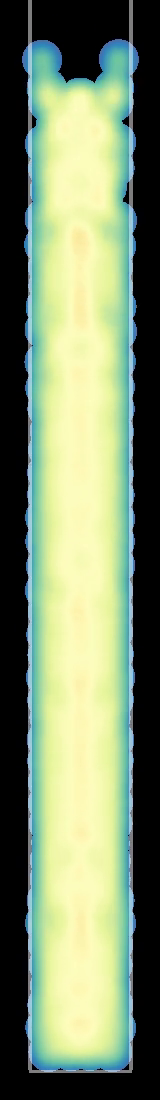
\includegraphics[width=\linewidth]{images/colpci4.png}
    \caption{$\abr{\rho}$ using \acs{pcisph}}
    \label{fig:col-pci}
  \end{subfigure}%
  \hspace{1cm}%
  \begin{subfigure}[t][0.1\linewidth]{0.25\linewidth}
    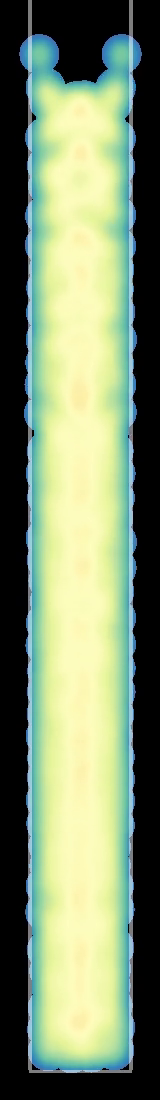
\includegraphics[width=\linewidth]{images/colopt4.png}
    \caption{$\abr{\rho}$ using \autoref{eq:incompressible-qp}}
    \label{fig:col-opt}
  \end{subfigure}\vspace{1cm}
  \caption{A colour-coded \ac{sph} reconstruction of the density field $\abr{\rho}$ using a conventional \ac{pcisph} pressure solver and using the method presented in this report are compared for a static water column at $t=1s$. Due to the large number of particles stacked vertically that require pressure to overcome gravity, this scene is challenging. Despite this, no significant compression can be observed. The \ac{qp} is in visual agreement with the solution obtained from the conventional solver, validating the result. Parameters are $N=200, \Delta t = 10^{-2}\text{s}, \nu=10^{-4}\text{Pa} \cdot \text{s}, \hbar=0.2\text{m}, \epsilon=10^{-3}\rho_0, \rho_0=1000\frac{\text{kg}}{\text{m}^2}$ on a $0.3\text{m}\times 5\text{m}$ domain.} 
  \label{fig:column-resting}
\end{figure}

\begin{figure}
  \centering
  \begin{subfigure}[t][0.1\linewidth]{0.9\linewidth}
    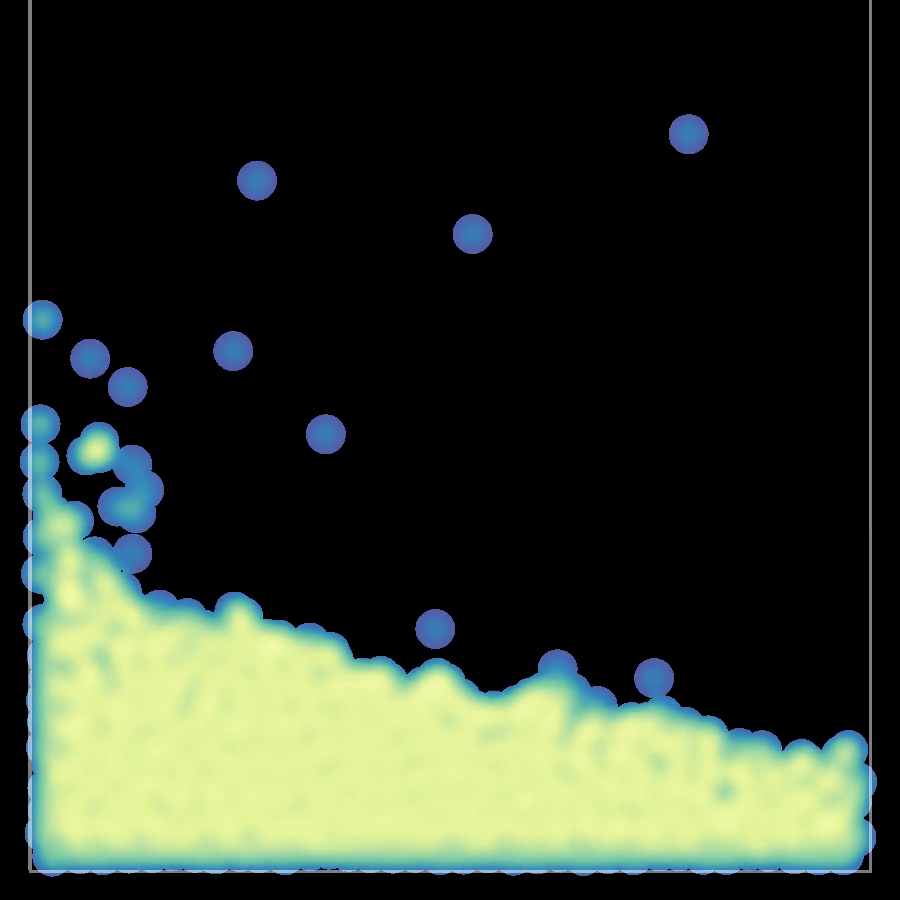
\includegraphics[width=\linewidth]{images/dynpci5.png}
    \caption{$\abr{\rho}$ using \acs{pcisph}}
    \label{fig:col-pci}
  \end{subfigure}%
  \vspace{1cm}
  \begin{subfigure}[t][0.1\linewidth]{0.9\linewidth}
    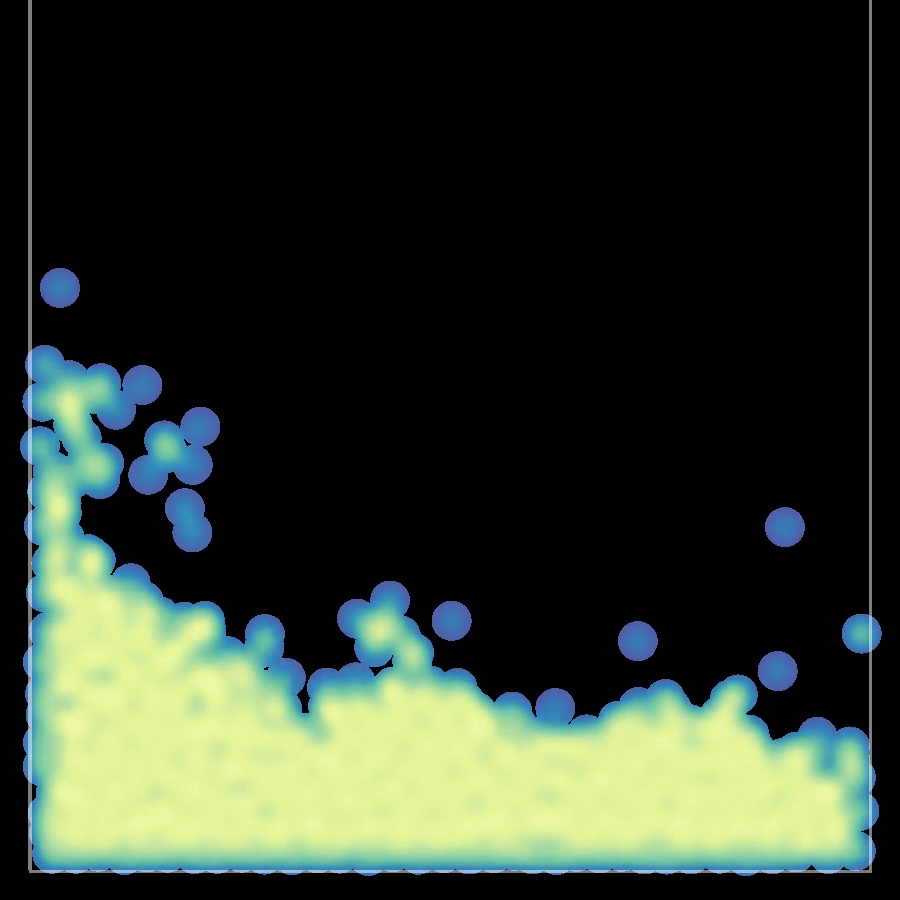
\includegraphics[width=\linewidth]{images/dynopt5.png}
    \caption{$\abr{\rho}$ using the \ac{qp} in \autoref{eq:incompressible-qp}}
    \label{fig:col-opt}
  \end{subfigure}\vspace{1cm}
  \caption{A colour-coded \ac{sph} reconstruction of the density field $\abr{\rho}$ using a conventional \ac{pcisph} pressure solver and using the method presented in this report are compared for a dynamic dam-break scenario at $t=5s$. The solution of the \ac{qp} is similar to that of the \ac{pcisph} solver, but shows slightly less intense splashing - whether this slight difference is an improvement in terms of not overshooting optimal pressures or a just a symptom of the system being chaotic is unclear. Parameters are the same as in \autoref{fig:column-resting}, but using a $2\text{m}\times 2\text{m}$ initial fluid sampling ($N=420$) in the bottom-left corner of a $4\text{m}\times 4\text{m}$ domain.} 
  \label{fig:dynamic-scene}
\end{figure}

\begin{figure}
  \centering
  \resizebox{\columnwidth}{!}{%
    \begin{tikzpicture}
      \begin{axis}[
        xlabel={$t$ ($\text{s}$)},
        ylabel={$p_\text{max}(t)$ ($\text{Pa}$)},
        grid=major,
        legend pos= north east,
        no markers,
        scale only axis,
        trim axis left,
        trim axis right,
        xmin=0, xmax=1,
      ]
        \addplot [color=red, thick] table[x=ts, y=pmaxo, col sep=comma] {pmaxdata.csv};
        \addlegendentry{$p_\text{max}$ of QP}
        \addplot [color=orange, thick] table[x=ts, y=pmaxc, col sep=comma] {pmaxdata.csv};
        \addlegendentry{$p_\text{max}$ of PCISPH}
      \end{axis}
    \end{tikzpicture}%
  }
  \caption{For the water column under hydrostatic pressure illustrated in \autoref{fig:column-resting}, the maximum pressure of each approach is plotted as a function of time for the first second of the simulation. The spike in pressure at $t\approx 0.1\text{s}$ is precisely the same for both independent solvers, confirming that this behaviour is expected of a \ac{sph}-discretization at the given spatial and temporal resolutions and is not an error in the implementation of either solver. The later trajectory of maximum pressures starts to differ, as numerical differences build up in a chaotic manner. This scneario highlights the benefit of the \ac{qp}-based solution that is optimal in an action-sense as a tool for the verification of correctness of other \ac{sph} based solvers when surprising results arise.} 
  \label{fig:pressure-graph}
\end{figure}

\begin{figure}
  \centering
  \resizebox{\columnwidth}{!}{%
    \begin{tikzpicture}
      \begin{axis}[
        xlabel={$t$ ($\text{s}$)},
        ylabel={$\rho$ ($\frac{\text{kg}}{\text{m}^2}$)},
        grid=major,
        legend pos= north east,
        no markers,
        scale only axis,
        trim axis left,
        trim axis right,
        xmin=0, xmax=2,
      ]
        \addplot [color=red, thick, dotted] table[x=ts, y=rhoavgo, col sep=comma] {rhoavgdata-dyn.csv};
        \addlegendentry{$\rho_\text{avg}$ of QP}
        \addplot [color=orange, thick, dotted] table[x=ts, y=rhoavgc, col sep=comma] {rhoavgdata-dyn.csv};
        \addlegendentry{$\rho_\text{avg}$ of PCISPH}

        \addplot [color=red, thick] table[x=ts, y=rhomaxo, col sep=comma] {rhoavgdata-dyn.csv};
        \addlegendentry{$\rho_\text{max}$ of QP}
        \addplot [color=orange, thick] table[x=ts, y=rhomaxc, col sep=comma] {rhoavgdata-dyn.csv};
        \addlegendentry{$\rho_\text{max}$ of PCISPH}
      \end{axis}
    \end{tikzpicture}%
  }
  \caption{The time evolution of average and maximum densities across the first $2\text{s}$ of the simulation of the dynamic dam-break scene illustrated in \autoref{fig:dynamic-scene} is shown for the \ac{pcisph} and \ac{qp} methods. Even initially, due to particle deficiency at the boundary the average density is below rest density $\rho_0=1000\frac{\text{kg}}{\text{m}^2}$, which highlights the significance of the inequality-based incompressibility constraint. Similar spikes in maximum density form as hydrostatic pressure is built up at around $t\approx 0.5\text{s}$ which exceed the error threshold $\epsilon$, highlighting the error incurred in the linearization of the incompressibility constraint in \autoref{eq:rho-change-non-pr} where an uncompressed predicted density does not result in an uncompressed measured density at the next time step, which is plotted here. Again, both solvers are in agreement.} 
  \label{fig:density-graph}
\end{figure}


\section{Alternative Formulations}
Two alternative formulations of the optimization problem that arose in the development of this report are particularly interesting, despite failing to produce the desired results, and will briefly be mentioned in the following.

\subsection{Non-Linear Incompressibility Constraint}\label{sec:nlp-attempt}
As observed in \autoref{fig:density-graph}, the use of a linearized incompressibility constraint in \autoref{eq:rho-change-non-pr}, while generally accurate, can cause significant discrepancies between densities at the next time step $\rho(t + \Delta t)$ and predicted densities including pressure accelerations $\rho^{**}(t+\Delta t)$ as defined in \autoref{eq:incompressibility-positive} at some individual particles, causing spikes in the maximum density that exceed the error threshold $\epsilon$. This can be avoided and an exact, density-invariant incompressibility constraint as originally derived from the continuity equation in \autoref{eq:source-rho-abs}, or an inequality-based variation which prevents clustering at the free surface, can be applied directly. 

Since predicted densities due to non-pressure accelerations are known (when viscous accelerations and gravity are integrated explicitly), given the pressures $\vek{p}$, the resulting pressure accelerations and therefore the total \ac{sph}-discretized acceleration in \autoref{eq:discretized-momentum} can be computed, allowing the computation of the exact positions of all particles at the next time step $\vek{x}(t+\Delta t, \vek{p})$ as a function of pressures. Indeed this is what is done in the \ac{qp} method after a minimizer $\vek{p}^*$ has been computed. This means that the densities $\rho(t+\Delta t)$ can be computed using \autoref{eq:density-estimate} from the subsequent positions $\mat{X}(t+\Delta t, \vek{p})$, which themselves are an affine function of unknown pressures $\vek{p}$. Unfortunately, due to the \ac{sph} kernel function taking particle positions as arguments, the exact densities $\rho(t+\Delta t)$ at the next time step are a non-linear function in pressures, since $\mat{X}(t+\Delta t, \vek{p})$ enters through the non-linear kernel function $W$. Also, since updated particle positions $\mat{X}(t+\Delta t, \vek{p})$ are required which might change the neighbour relations captured by neighbour sets $\mathcal{N}_i$ (\autoref{eq:neighbour-set-def}), neighbourhood search has to be performed in a larger radius (at least an increase in radius of $h$ according to the \ac{cfl} condition in \autoref{eq:cfl}) to account for particles entering or exiting another particle's kernel support radius in the current time step. This increase in search radius results in larger neighbour sets $\mathcal{N}_i$, the cardinalities of which scale in the search radius to the $d^{\text{th}}$ power in $d$ dimensions for a typical particle sampling, massively increasing computational cost. 

Furthermore, the inequality constraint:
\begin{equation}
  \abr{\rho_i}(t+\Delta t, \vek{p}) \leq \rho_0
\end{equation}
is non-linear in pressures as previously mentioned, meaning that the resulting optimization problem becomes an \ac{nlp} instead of a \ac{qp} and becomes much harder to solve, to the point where an experimental implementation using IPOPT \cite{ipopt} failed to converge to a feasible point. If such a constraint were computationally feasible to implement, it could very much be preferable to the presented, linearized approach.

\subsection{Two-Stage Problem with Minimum Tolerance}
The choice of the error tolerance $\epsilon$ was left as a parameter in the presented approach, but an error tolerance on the incompressibility constraint that is as close to zero as possible is desired. It was attempted to first minimize a scalar $\tilde{\epsilon} \in\mathds{R}$ subject to the same constraints as in \autoref{eq:incompressible-qp} except that the constraint $\tilde{\epsilon} \geq 0$ was added, meaning that the least feasible error threshold was computed before using the resulting $\tilde{\epsilon}^*$ in the suggested \ac{qp}, resulting in a two-stage approach with minimum feasible incompressibility violation. Unfortunately, if a linearized density invariance constraint is used as suggested, $\tilde{\epsilon}^*=0$ can always be achieved and the optimal value of $\epsilon$ is trivially zero, although a higher value might still decrease the computational cost of finding the solution to the \ac{qp}. It is suspected that the same would not be the case if an exact incompressibility constraint as described in \autoref{sec:nlp-attempt} was used and instead the truly optimal pressure field with the smallest possible maximum error would be found, which would represent the holy grail of \ac{sph} pressure computation. Unfortunately the resulting \ac{nlp} could not be solved in experiments, as already mentioned.

\section{Conclusion}
In this report, the problem of Lagrangian, particle-based simulation of low-viscosity, incompressible Newtonian fluids on macroscopic scales was described, the \acf{ppe} was introduced as a way to encode incompressibility and \ac{sph} was derived as a scheme for discretizing the resulting Navier-Stokes equations, including discussions of differential operators on discretized fields. This lead to the setting of \ac{sph}-based pressure computation for incompressible fluids, where problematic boundary effects at the free surface were described and the introduction of inequality constraints on pressures and compressions was suggested to fix the resulting problems, leading from a system of linear equations to the search of a feasible pressure vector. This reformulation was then related to approaches implemented by existing \ac{sph} pressure solvers to argue that the suggested inequality constraints were indeed desired. From this, existing approaches were modelled as ill-posed optimization problems in order to explain instabilities that arise in conventional solvers, which were assumed to search for any feasible pressure field, whereas the least feasible pressure field is desired, resulting in different behaviour depending on solver implementation and initialization in particular. This notion of a \textit{least} pressure field was then defined using Gau\ss's principle of least constraint to derive an objective function that fixes the reliance on conservative initialization and represents a physically valid, optimal pressure field. This resulted in a \ac{qp} that was analysed and implemented using an \ac{ipm} approach to be compared to a conventional pressure solver. The solvers were found to be in agreement, substantiating the validity and robustness of the suggested approach, but leaving the massively decreased performance compared to conventional, parallel solvers (by multiple orders of magnitude for most scenes), as well as the problem of eliminating the null-space of the objective functions open. Variations of the suggested optimization problem were discussed that could improve accuracy but constitute much more difficult, non-linear problems. 

% \bibliographystyle{IEEEtran}
% \bibliography{refs}
\printbibliography

\section*{Acronyms}
\begin{acronym}[PCISPH] % <- longest label
  \acro{sph}[SPH]{Smoothed Particle Hydrodynamics}
    \acro{ppe}[PPE]{Pressure Poisson Equation}
    \acro{lp}[LP]{Linear Program}
    \acro{qp}[QP]{Quadratic Program}
    \acro{qps}[QPs]{Quadratic Programs}
    \acro{nlp}[NLP]{Non-Linear Program}
    \acro{lcp}[LCP]{Linear Complementarity Problem}
    \acro{ncp}[NCP]{Non-Linear Complementarity Problem}
    \acro{pdes}[PDEs]{Partial Differential Equations}
    \acro{ode}[ODE]{Ordinary Differential Equations}
    \acro{cfl}[CFL]{Courant-Friedrichs-Lewy}
    \acro{iisph}[IISPH]{Implicit Incompressible SPH}
    \acro{pcisph}[PCISPH]{Predictive-Corrective SPH}
    \acro{pbf}[PBF]{Position Based Fluids}
    \acro{dfsph}[DFSPH]{Divergence-free SPH}
    \acro{cg}[CG]{Conjugate Gradients}
    \acro{nncg}[NNCG]{Non-Smooth Nonlinear Conjugate Gradient}
    \acro{ipm}[IPM]{Interior Point Method}
\end{acronym}


\end{document}